\documentclass[hidelinks,12pt,a4paper]{article}
\usepackage[utf8]{inputenc}
\usepackage{amsmath}
\usepackage{amsfonts}
\usepackage{amssymb}
\usepackage{wasysym}
\usepackage[superscript,biblabel]{cite}
\usepackage{url}
\usepackage{graphicx}
\usepackage{csquotes}
\usepackage{placeins}
\usepackage{setspace}
\usepackage{hyperref}
\usepackage{float}
\usepackage{titlesec}
\usepackage{anyfontsize}
\usepackage{import}
\usepackage[font=scriptsize]{caption}

\graphicspath{ {images/} }

\onehalfspacing
\titleformat*{\section}{\Large}
\titleformat*{\subsection}{\normalsize}

\titlespacing{\section}{0pt}{24pt}{0pt}
\titlespacing{\subsection}{0pt}{18pt}{0pt}

\title{%
  \LARGE Underground Pumped Hydroelectric Storage:\\
  \LARGE A Feasibility Study\\
  \bigskip
  \normalsize [Version: DRAFT 0.0.2]
}

\author{\large Eric Chaves}
\date{\large \today}


\begin{document}
\maketitle
\setlength{\parindent}{1em}
\setlength{\parskip}{1em}


\renewcommand{\abstractname}{Abstract}
\begin{abstract}
In this report, we determine that it is feasible for an energy storage technology called Underground Pumped Hydroelectric Storage to play a fundamental role in our fight against climate change.

We explain that energy sources like wind and solar are expected to replace fossil fuels, which will increase the variablility of our grid's supply. And this will drive an exponential growth in demand for energy storage.

We argue that underground pumped hydro technology could provide plentiful energy storage at the most affordable cost. Over long time frames of 40-80 years, this solution could be an order of magnitude cheaper than chemical battery solutions like Lithium Ion.

Recent studies have concluded that stationary energy storage demand is expected to grow exponentially and require half a trillion dollars of investments over the next two decades. We believe that underground pumped hydro could capture some of this market from Lithium Ion battery installations. We suggest further exploration of underground pumped hydro technology. And we suggest immediate development of the technology on sites which may be deemed suitable for profitable installations.

\end{abstract}

\pagebreak[1]

\renewcommand{\baselinestretch}{0.75}\normalsize
{\footnotesize
  \tableofcontents
}
\renewcommand{\baselinestretch}{1.5}\normalsize

\pagebreak[4]
\section{Introduction}
Climate change poses a dire threat to humanity. The research is clear: If we do not immediately mitigate this risk, climate damages will escalate beyond our control.

In this report, we will examine why it will be critical in our fight against climate change to build an enormous capacity of energy storage in the coming decades. We will then advocate for a particular technology called Underground Pumped Hydro Energy Storage. We will demonstrate that this technology has unexplored potential for providing plentiful energy storage at the most affordable cost.

\subsection{Climate Change: Risk and Opportunity}
The 2018 US National Climate Assessment Report concludes that if we do not mitigate climate change, we face “substantial damages to the economy, environment, and human health over the coming decades.” \cite{NationalClimateAssessmentReport} This is not a political issue. Even if health and environmental factors are omitted from discussion, projected economic costs are a sufficient cause on their own to justify urgent climate investments.

According to a report by The Universal Ecological Fund, by the next decade, climate damages will cost the United States \$360 Billion a year on average. That's half of the expected growth of the economy. \cite{TheEconomicCaseForClimateActionInTheUnitedStates} The report affirms that “The benefits of taking climate action outweigh the escalating economic losses and health damages.” \cite{TheEconomicCaseForClimateActionInTheUnitedStates} Plain and simple, it is cheaper to deal with climate change than to ignore it.

\subsection{Green New Deals: Cities Aim for 100\% Renewable Energy by 2050}
“There’s been a global culture shift around clean energy,” \cite{TheSolutionsProject2018ImpactReport} concludes The Solutions Project, an organization whose board includes Mark Jacobson, a professor of civil and environmental engineering at Stanford. The Solutions Project (TSP) reports that: \cite{TheSolutionsProject2018ImpactReport}

{\footnotesize
\begin{itemize}
    \item Hundreds of major companies have committed to go 100\% renewable.
    \item 70\% of people now “agree that we should produce 100\% of our electricity from renewable sources in the near future.”
    \item Six cities are already running on 100\% renewable energy, and over 100 U.S. cities have made the 100\% commitment.
\end{itemize}
}

As depicted in the map below, over a hundred cities across the U.S. have drafted their own “Green New Deal” promises, pledging to become carbon neutral by 2050. These cities include San Francisco \cite{SFNetZeroBy2050} and New York. \cite{ActionOnGlobalWarmingNYCsGreenNewDeal} In this paper, we will use these two cities as case studies in order to depict how proposed solutions might work for these real use cases.

\begin{figure}[ht!]
    \centering
    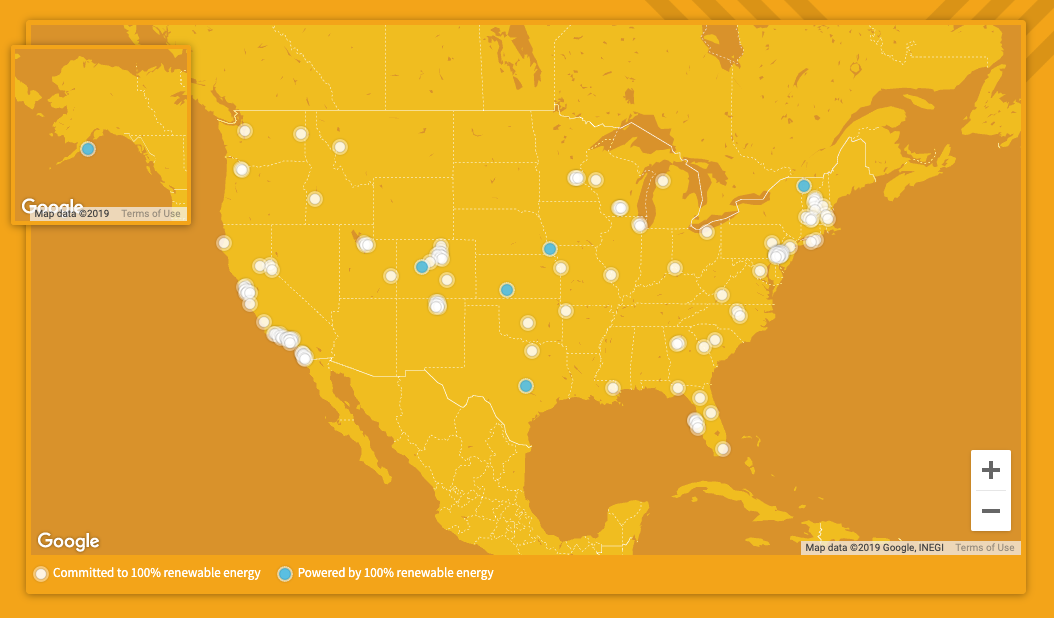
\includegraphics[width=1\textwidth]{over-100-cities-go-100-green.png}
    \caption{The Solutions Project - cities pledging zero carbon by 2050 \cite{TheSolutionsProject2018ImpactReport}}
\end{figure}
\FloatBarrier


Before Mark Jacobson joined The Solutions Project, he co-authored a report in 2015 which concluded that we can and should convert the United States to 100\% renewable energy by 2050. In the report (Jacobson report), he says this transition would be, “technically and economically feasible with little downside,” \cite{100PercCleanAndRenewableEnergyBy2050} and that the transition would provide massive benefits including: \cite{100PercCleanAndRenewableEnergyBy2050}

{\footnotesize
\begin{itemize}
    \item A reduction of each state’s end-use power demand by about 39\%
    \item A net gain of 2 million additional long term jobs
    \item Saving tens of thousands of annual premature deaths related to air pollution
    \item Saving an estimated \$2-\$7 trillion per year in 2050 global warming costs to the world due to U.S. emissions
    \item Saving each U.S. resident \$260 per year in energy costs (\$2013 dollars)
\end{itemize}
}

By quantifying and explaining the net benefits of going carbon neutral, the Jacobson report said it hoped to “reduce social and political barriers to implementing clean-energy policies.” \cite{100PercCleanAndRenewableEnergyBy2050}

In writing our report, we take inspiration from Jacobson's cause-driven research. In our report, we intend to highlight a particular technology which could solve a troubling problem with projected renewable energy growth. This technology, called Underground Pumped Hydro Energy Storage, or UPHS, could be our best hope to solve a looming shortage of energy storage. If this shortage is not covered, it will hinder future expansions of wind and solar energy.

\subsection{Introducing Underground Pumped Hydro Energy Storage}
UPHS was thoroughly researched and validated in the 1980s. But it seems the idea has been largely forgotten since. In our report, we will resurface the conclusions of this past research and show how UPHS might play a critical role in our fight against climate change.

Our report will first discuss Pumped Hydro Energy Storage in general (see explainer below: “What is Pumped Hydro?”).

Then, we will focus specifically on underground pumped hydro (UPHS) which is a variation of pumped hydro energy storage (PHS). Citing existing research, we will argue that UPHS is a promising alternative to today's energy storage solutions.

Even though UPHS has never been built on a large scale, research has shown it to be technically feasible and cost competitive. And it has a lower ecological footprint than traditional PHS which could prove invaluable for surviving the gauntlets of development approvals which often doom traditional PHS projects.

% \subsection{The Race to 100\% Clean Electricity by 2050}
\subsection{San Francisco and New York City Commit to Green New Deals}
San Francisco and New York City have both recently pledged that their cities would transition to 100\% clean electricity by 2050. \cite{SFNetZeroBy2050} \cite{ActionOnGlobalWarmingNYCsGreenNewDeal}

New York City's Green New Deal is outlined in the “A Livable Climate” section of their “OneNYC 2050” report published in 2019. Their report promises:

\begin{displayquote}
“Our multifaceted strategy for action is ambitious and far-reaching — as it must be....It will require innovation to find less expensive and more effective solutions; creative financing and financial investment; and partnerships across communities, sectors, geographies, and all levels of government.” \cite{OneNYC2050FullReport} -- OneNYC 2050 Report
\end{displayquote}

The NYC report acknowledges the need for increased energy storage. It states, “[deployment of wind and solar power] must expand rapidly in the next 20 years, and will need to be complemented by a significant expansion in energy storage.” \cite{OneNYC2050FullReport} It states further, “Energy storage resources will be required to balance the intermittent nature of renewable power generation, and we want to have 500 MW of storage available by 2025.”

500 MW is an ambitious goal for New York City considering that as of 2017, they only had 5 MWh of storage\cite{NYEnergyStorageTargetTheJourneyNotTheDestination}. Yet, even if NYC met this goal, it would still provide only a 2.8\% buffer for their total power usage (See Appendix). As we'll see below, this may not be enough power storage to support a large increase of wind and solar generation.

San Francisco also recently published a technical report which outlines their roadmap to achieve net zero emissions by 2050. \cite{Focus2030APathwaytoNetZeroEmissions}. “Every generation is defined by how they tackled a seemingly-insurmountable obstacle, and climate degradation is our generational marker,” said San Francisco Supervisor Ahsha Safaí as the city announced their commitment for net zero emissions by 2050.\cite{SanFranciscoMayor100PercentRenewableElectricity}

San Francisco's report only briefly mentions their future energy storage needs, but other research offers more detail. A 2017 report by the Bay Area Council Economic Institute (BACEI report) discusses California's energy storage needs in general:

\begin{displayquote}
“The need for energy storage and the energy storage market are growing rapidly as renewable generation, energy policies, and greenhouse gas reduction goals impact how the grid needs to be managed.”\cite{EnergyStorageCaliforniaClimateandEnergyGoals} --  Bay Area Council Economic Institute
\end{displayquote}

According to the report, in order for California to reach their target of 50 percent renewable energy by 2030, the state will need about 2.2 GW of additional energy storage capacity to add to their existing 4.2 GW (as of 2017).\cite{EnergyStorageCaliforniaClimateandEnergyGoals}


Using San Francisco and New York City as case studies, this report will examine how underground pumped hydro energy storage could help large cities meet their growing demand of energy storage. We will assess the enormous energy storage capacity needed to achieve the city's promised goals of 100\% renewable energy. And we will advocate that UPHS may be the cities' best option to supply their required energy storage volume.

\pagebreak[1]
\section{Why Energy Storage?}
Renewable energy sources like wind and solar have matured into a small but significant share of the energy market. These renewables are expanding rapidly, helping reduce the greenhouse gases which contribute to climate change. But even as a small market, these new energy sources have caused a troublesome side-effect on our energy supply. Since the sun doesn’t always shine and the wind doesn’t always blow, renewables increase the variability of our net power supply.

This simple effect has a complicated impact on our energy grid. Our grid cannot tolerate variability. To avoid surges or rolling blackouts, the grid must maintain a constant balance of supply and demand. And with our current infrastructure, there is very little wiggle room.

It has been well reported for years that there is an important correlation between energy storage and renewable electricity. In a 2010 technical report, the U.S. National Renewable Energy Laboratory (NREL) concluded: “It is clear that high penetration of variable generation increases the need for all flexibility options including storage, and it also creates market opportunities for these technologies.” \cite{TheRoleOfEnergyStorageWithRenewableElectricityGeneration}

These market opportunities become clear when we examine the costly inefficiencies that arise from a lack of energy storage. Even at today's levels of variable generation, curtailment is becoming an expensive problem. This issue is explained in detail by the BACEI report referenced earlier:

\begin{displayquote}
“During overgeneration conditions primarily driven by an oversupply of solar, the power being generated is in excess of real-time demand. This leads to what is referred to as the “duck curve”...which projects the supply-demand gap produced by variable power. The “belly” of the duck shows lowest net load, when solar generation is highest, followed by the afternoon upward ramp or “neck” of the duck. In the absence of an ability to store that excess energy, overgeneration is currently being addressed by curtailment—the purposeful reduction of renewable generation in order to keep the grid stable. This is done by decreasing the output from a wind or solar plant or disconnecting the plant altogether. Curtailment can be done for large renewable power plants but not for smaller or distributed systems like rooftop solar.” \cite{EnergyStorageCaliforniaClimateandEnergyGoals}
\end{displayquote}

\begin{figure}[ht!]
    \centering
    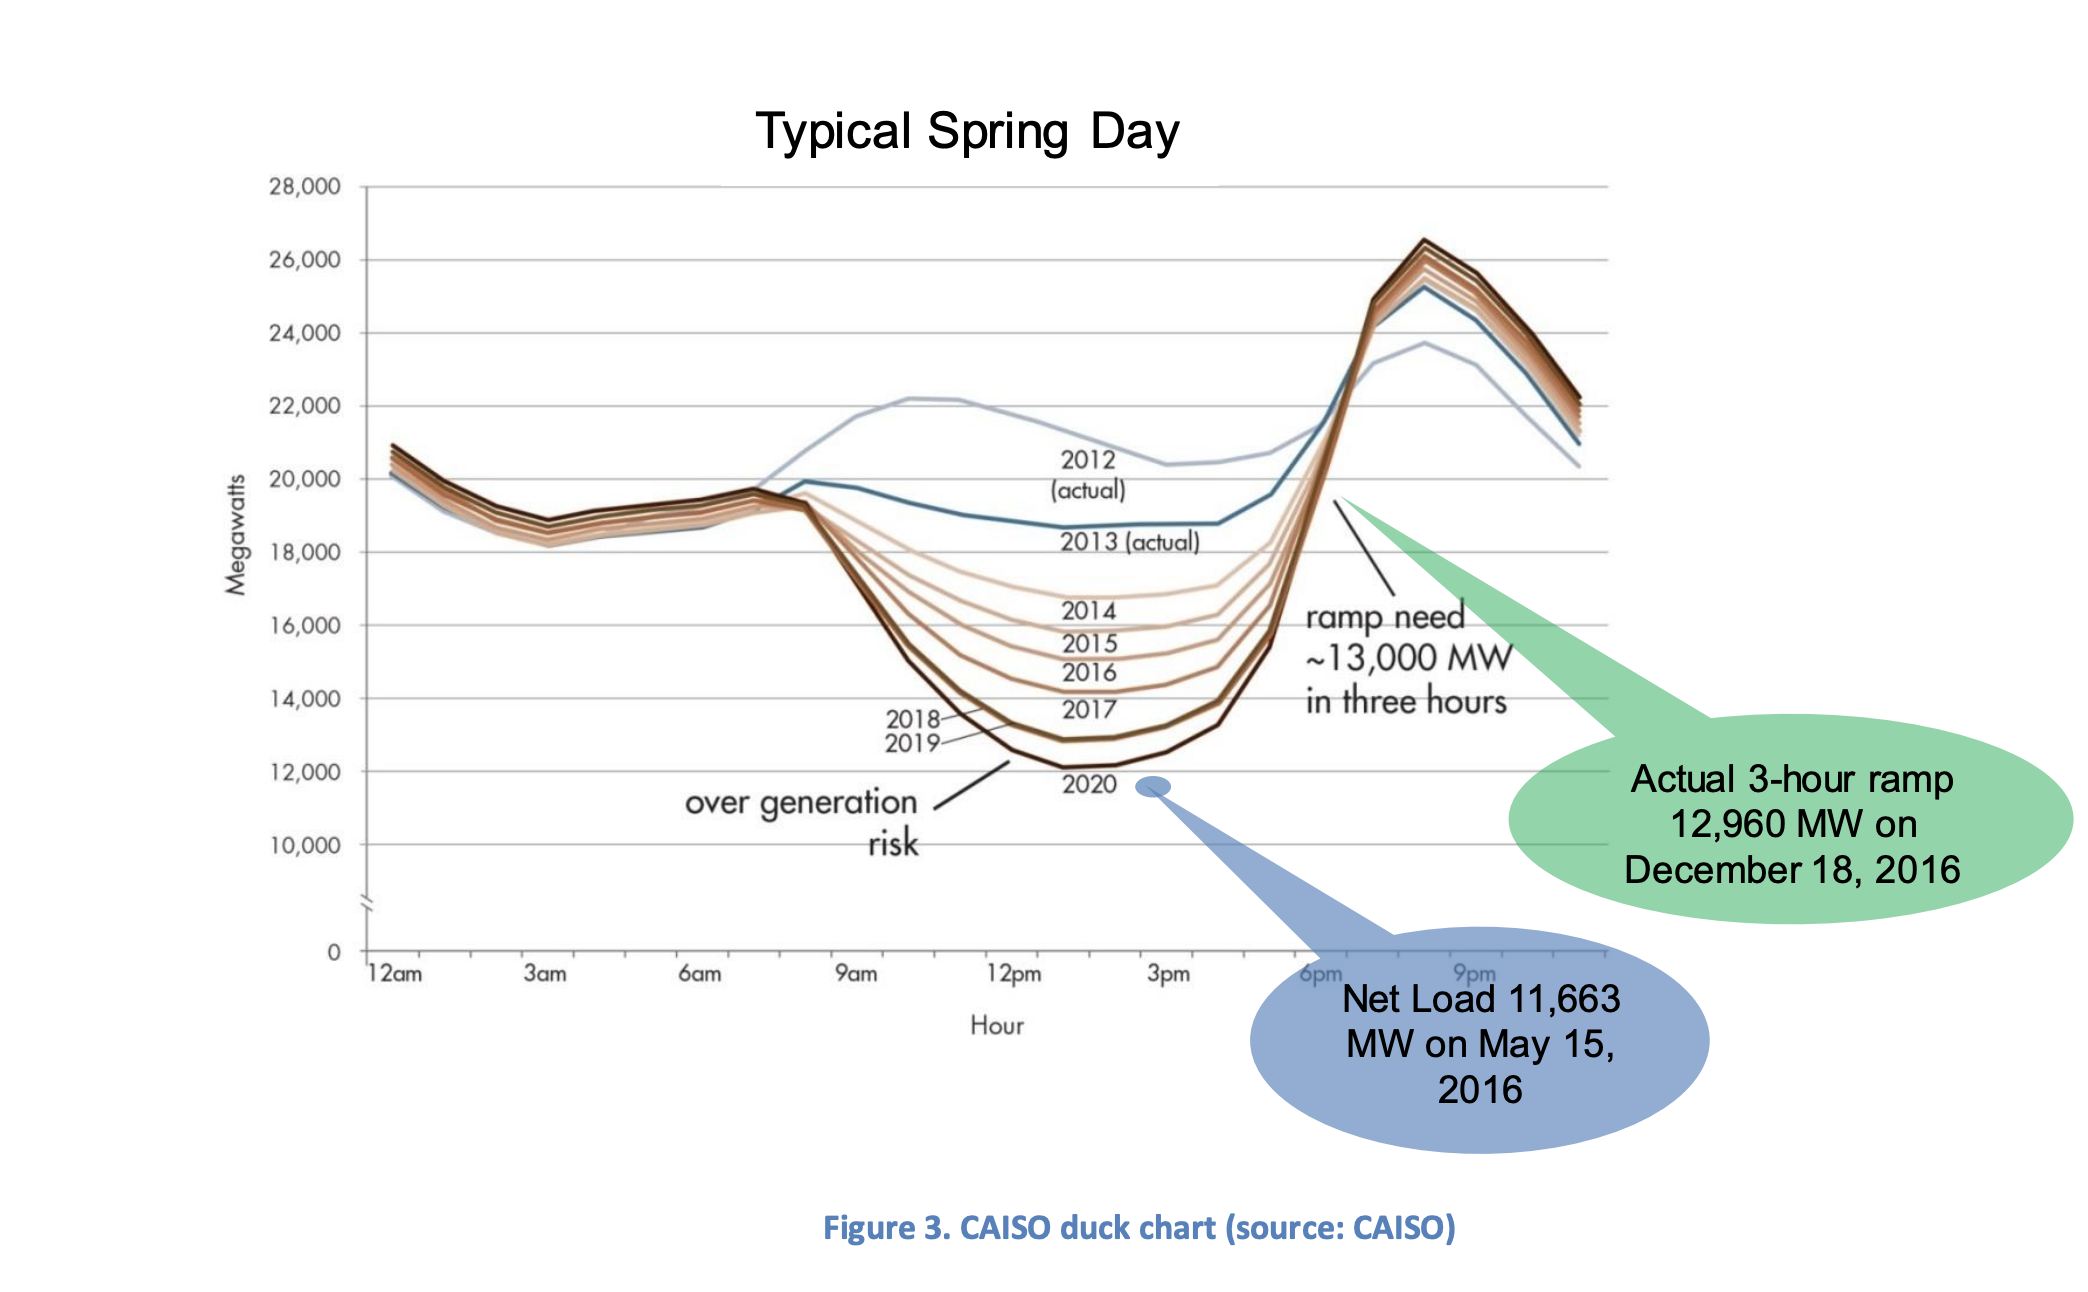
\includegraphics[width=0.75\textwidth]{california-duck-curve.png}
    \caption{Graph illustrating a “duck curve.” Source: California ISO \cite{UsingRenewablesToOperateLowCarbonGrid}}
\end{figure}
\FloatBarrier

Without sufficient energy storage capacity, our grid must instead rely on so called peaker plants in order to avoid rolling blackouts during peak loads. Fossil fuel burning peaker plants are inefficient and expensive because they must remain inactive most of the time and kick into production only when the grid's demand spikes to peak load. Energy storage solutions are cleaner alternatives, and due to a drop in battery prices, they are becoming price competitive as well. The market is beginning to respond to this new reality. Initiatives across the United States are beginning to replace these polluting peaker plants with chemical battery facilities. \cite{StorageWillReplaceThreeCaliforniaGasPlants, NewYorkMovesToPhaseOutOlderPeakingPlants}

\subsection{The State of our Energy Storage}
In the United States, our energy storage capacity is only 2.5\% of total electric power. For comparison, 10\% of delivered power in Europe and 15\% of delivered power in Japan are cycled through energy storage facilities. \cite{USGridEnergyStorageFactsheet}

With such a low capacity of energy storage, we are ill prepared to handle an increase in variable energy generation. As mentioned above, some initiatives have begun to address local energy storage problems with chemical battery facilities. But this is on a very small scale.

Looking at the big picture, nearly all of our storage capacity (94\%) is generated from pumped storage. \cite{ElectricStorageCapacityInTheUnitedStates} Chemical batteries on the other hand, are less than 5\% of the market; only about 0.1\% of our grid's power can be stored in chemical batteries today.

\begin{figure}[ht!]
    \centering
    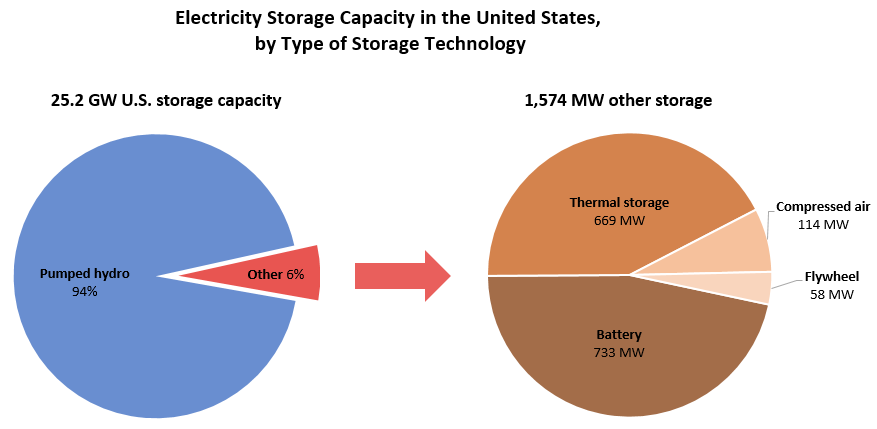
\includegraphics[width=0.75\textwidth]{energy-storage-pie-charts.png}
    \caption{Illustration from EPA.gov \cite{ElectricStorageCapacityInTheUnitedStates}}
\end{figure}
\FloatBarrier

Despite technological advances in chemical battery efficiency, they are not cost competitive with pumped hydro at large scales. This will be explained in more detail below.

\subsection{What is Pumped Hydro?}
Pumped Hydro Storage (PHS) is a system comprised of two large water reservoirs with a difference in elevation between them. This system creates a battery from the gravitational potential difference of water pumped between them. During periods of high electricity demand, power is generated by dropping water down through a hydropower dam turbine. During periods of low demand, the upper reservoir is recharged by using lower-cost electricity to pump water back up.

Pumped hydro energy storage is affordable and efficient. PHS plants can last half a century or more, and their round-trip efficiencies can exceed 80\%. \cite{USGridEnergyStorageFactsheet}

The BACEI report summarizes:

\begin{displayquote}
“For bulk or grid-scale power management applications, pumped storage is widely considered to be the most demonstrated and most economic technology, with the capacity to provide over a gigawatt of power over durations of 12 hours or more.” \cite{EnergyStorageCaliforniaClimateandEnergyGoals} -- BACEI report
\end{displayquote}

\begin{figure}[ht!]
    \centering
    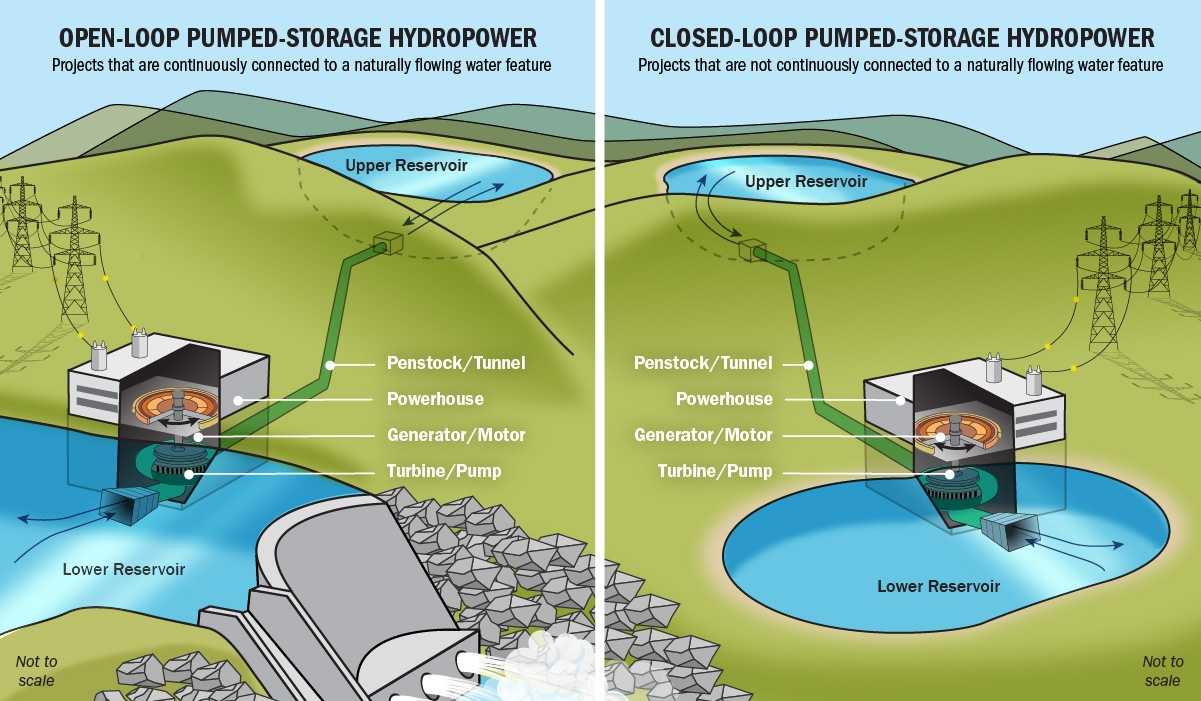
\includegraphics[width=1.00\textwidth]{111148-5000-wpto_pumped_storage_illustration_0.jpg}
    \caption{Illustration from energy.gov. \cite{EnergyGovPumpedStorageHydropower}}
\end{figure}
\FloatBarrier

As of 2017, the U.S. had a total of about 20 GW of conventional pumped storage hydropower spread across more than 40 facilities. \cite{EnergyStorageCaliforniaClimateandEnergyGoals} But as we'll see in the following sections, demand for energy storage capacity is expected to rise exponentially.


\subsection{Keeping up with Wind and Solar}
According to the U.S. Energy Information Administration (EIA), renewable energy resources such as solar and wind are currently the fastest growing sources of U.S. electricity generation. \cite{EIAForecastsRenewables}

\begin{figure}[ht!]
    \centering
    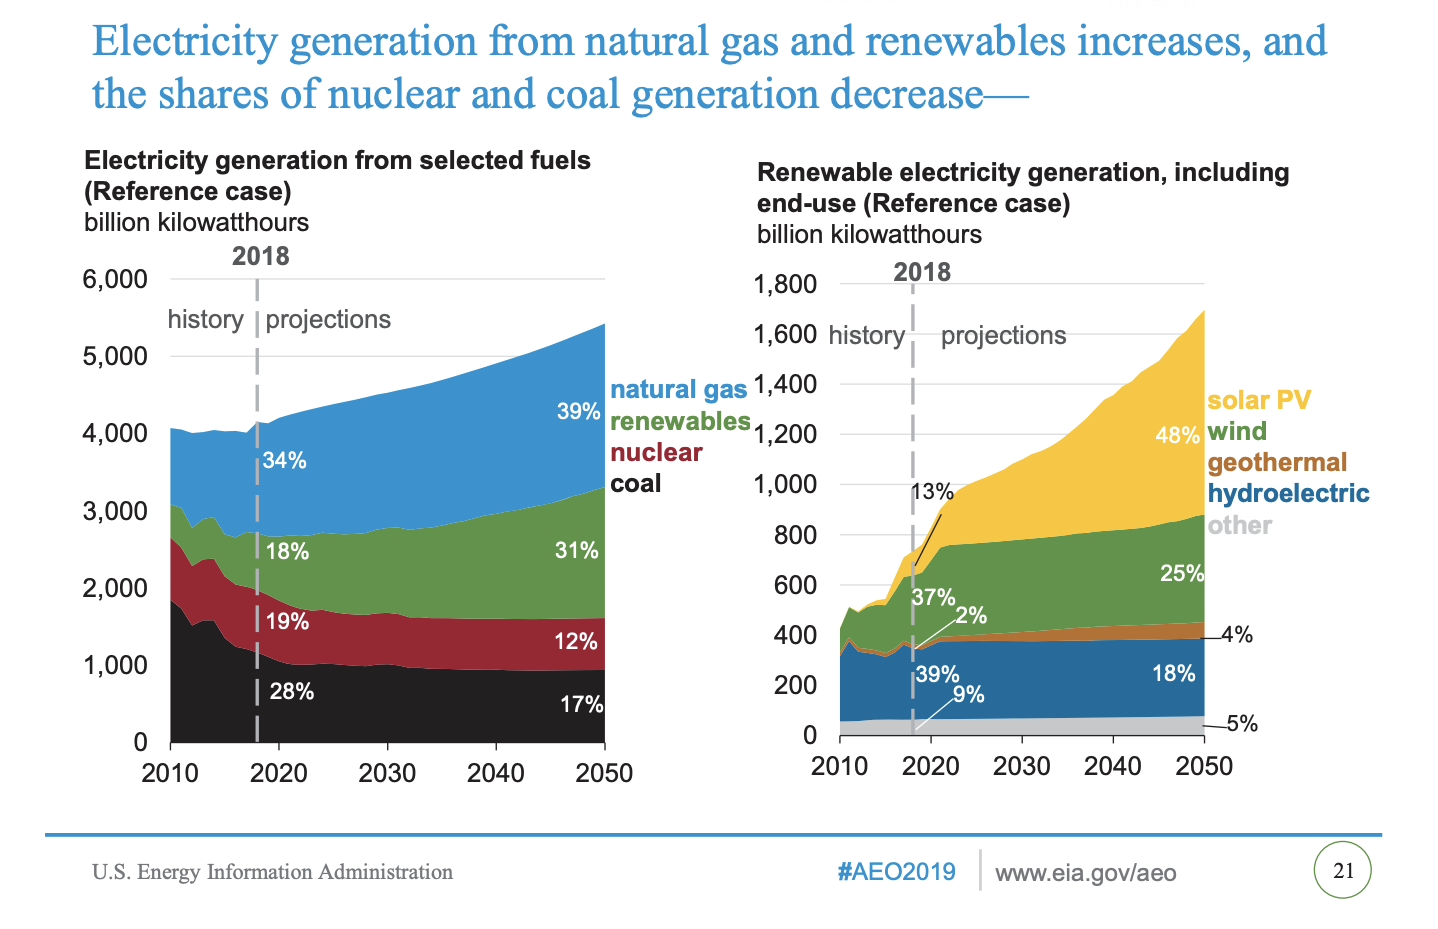
\includegraphics[width=1.00\textwidth]{EIA-2019-energy-generation-projections.png}
    \caption{Illustration from a 2019 EIA.gov report. \cite{EIAForecastsRenewables}}
\end{figure}
\FloatBarrier

As illustrated in the graph above, the EIA report projects that renewable energy will nearly double its market share by 2050.

This should be wonderful news for green energy advocates. But there's a problem. Because wind and solar energy add so much variability to grid demand, this projected growth might not even be possible without an accompanied growth of energy storage capacity. And this problem gets exponentially worse as renewable energy captures larger market share.

\subsection{The Uphill Battle to 100\% Renewable Energy}
“The sun doesn’t always shine and the wind doesn’t always blow.” This truism is an oft-used reminder of renewable energy variability. Let's consider what it means in practice. Imagine if we relied only on solar energy, how much energy storage would we need? On each sunny day we would need to capture almost twice the demand of our entire grid so we could store half to use at night. And what about cloudy days?

A 2018 article from the MIT Technology Review answers these questions with some real numbers. Taking California as an example, the article concludes that our future energy storage needs will be astronomically expensive, especially if we rely on chemical batteries. The article cites a 2016 analysis \cite{EnergyStorageDecarbonizingElectricity} in which researchers found “steeply diminishing returns when a lot of battery storage is added to the grid.” \cite{TheTwoPointFiveTrillionReasonWeCantRelyOnBatteries}


\subsection{Lithium-ion Energy Storage: A Good First Step, but Bad at Scale}
As prices drop for lithium-ion batteries, chemical battery storage has proved to be a viable replacement for fossil-fuel peaker plants. This is an important next step for energy storage growth; each retired peaker plant will save money and reduce pollutants. But unfortunately, chemical batteries are not well suited to solve energy storage on large scales.

The MIT Technology Review article explains that, “much beyond this role [of replacing peaker plants], batteries run into real problems.” \cite{TheTwoPointFiveTrillionReasonWeCantRelyOnBatteries} The article continues, “Not only is lithium-ion technology too expensive for this role, but limited battery life means it’s not well suited to filling gaps during the days, weeks, and even months when wind and solar generation flags.” \cite{TheTwoPointFiveTrillionReasonWeCantRelyOnBatteries} Quoting MIT researcher Jesse Jenkins, the article explains that “when renewables reach high levels on the grid, you need far, far more wind and solar plants to crank out enough excess power during peak times to keep the grid operating through those long seasonal dips. That, in turn, requires banks upon banks of batteries that can store it all away until it’s needed....And that ends up being astronomically expensive.” \cite{TheTwoPointFiveTrillionReasonWeCantRelyOnBatteries}

\subsection{Lithium-ion Energy Storage: Projected Costs for California Case Study}

California is already on track to get 50 percent of its electricity from clean sources by 2020, and the state is considering a bill pushing them to 100 percent by 2045. The MIT Technology Review article examines the correlated costs of battery storage which would be needed to support this growth.

\begin{figure}[ht!]
    \centering
    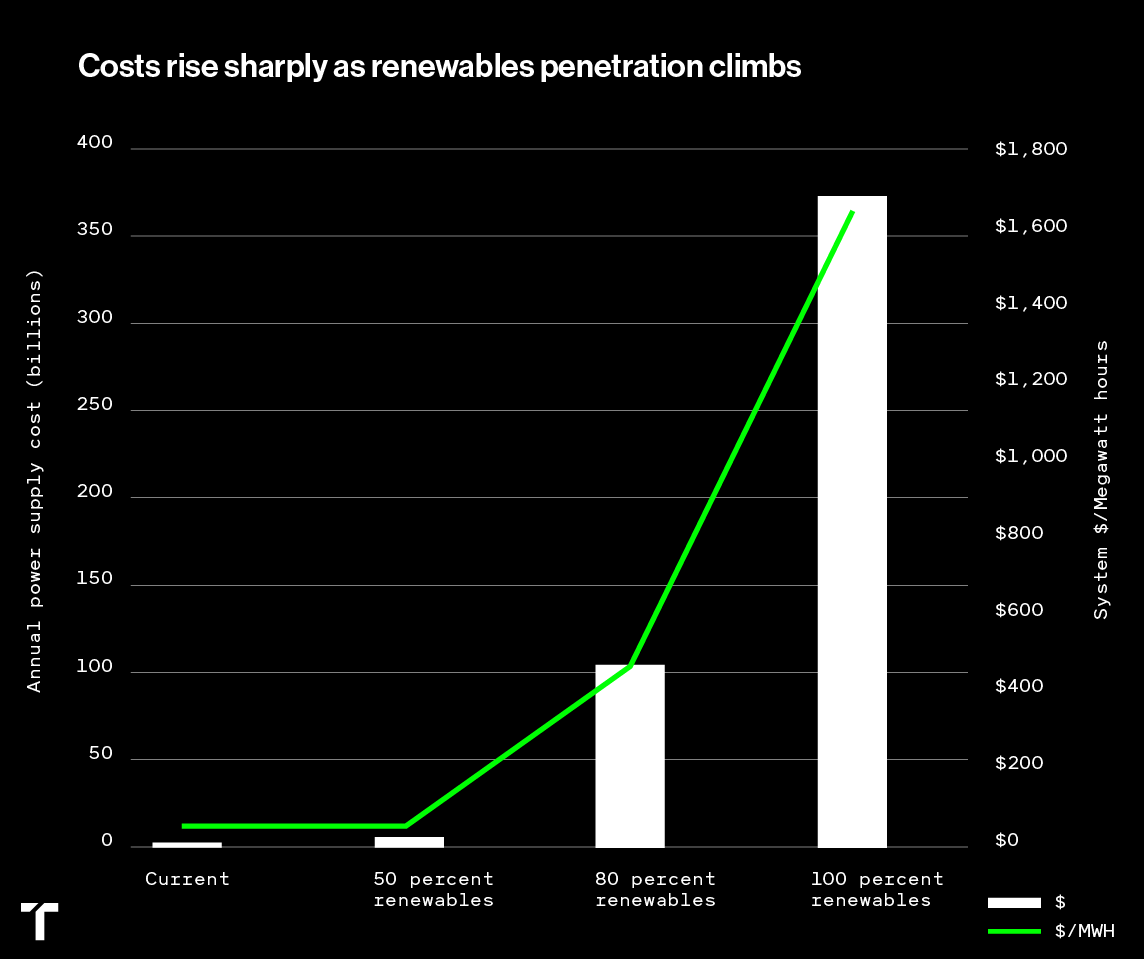
\includegraphics[width=0.7\textwidth]{batterystorage-02_0.png}
    \caption{Illustration from technologyreview.com. \cite{TheTwoPointFiveTrillionReasonWeCantRelyOnBatteries}}
\end{figure}
\FloatBarrier

As depicted in the graph above, if California's roadmap depended on current battery technology, their energy storage costs would rise exponentially, from \$49 per megawatt-hour of generation at 50 percent to \$1,612 at 100 percent. And that's assuming lithium-ion batteries will cost roughly a third what they do now. This kind of system could cost California more than \$2.5 trillion just to meet 80\% of demand with wind and solar. \cite{TheTwoPointFiveTrillionReasonWeCantRelyOnBatteries} At these outrageous prices, chemical batteries will not likely be a feasible solution to support the future grid-scale energy storage.

\subsection{An Astronomical Expense, but Cheaper Than Nothing}
If chemical batteries can't offer a scalable solution to fill market demand for energy storage, what technologies will?

According to a market report by Wood Mackenzie, U.S. Energy Storage deployments nearly doubled in 2018, growing 80\% from 2017. \cite{USEnergyStorageMonitor2018YIRAndQ12019} The authors state: “The [U.S. Energy storage] market will double from 2018 to 2019, then nearly triple from 2019 to 2020.” Looking further, the “U.S. energy storage annual deployments will reach 4.4 GW by 2024.” This signals a 14-fold growth between 2018 and 2024.

\begin{figure}[ht!]
    \centering
    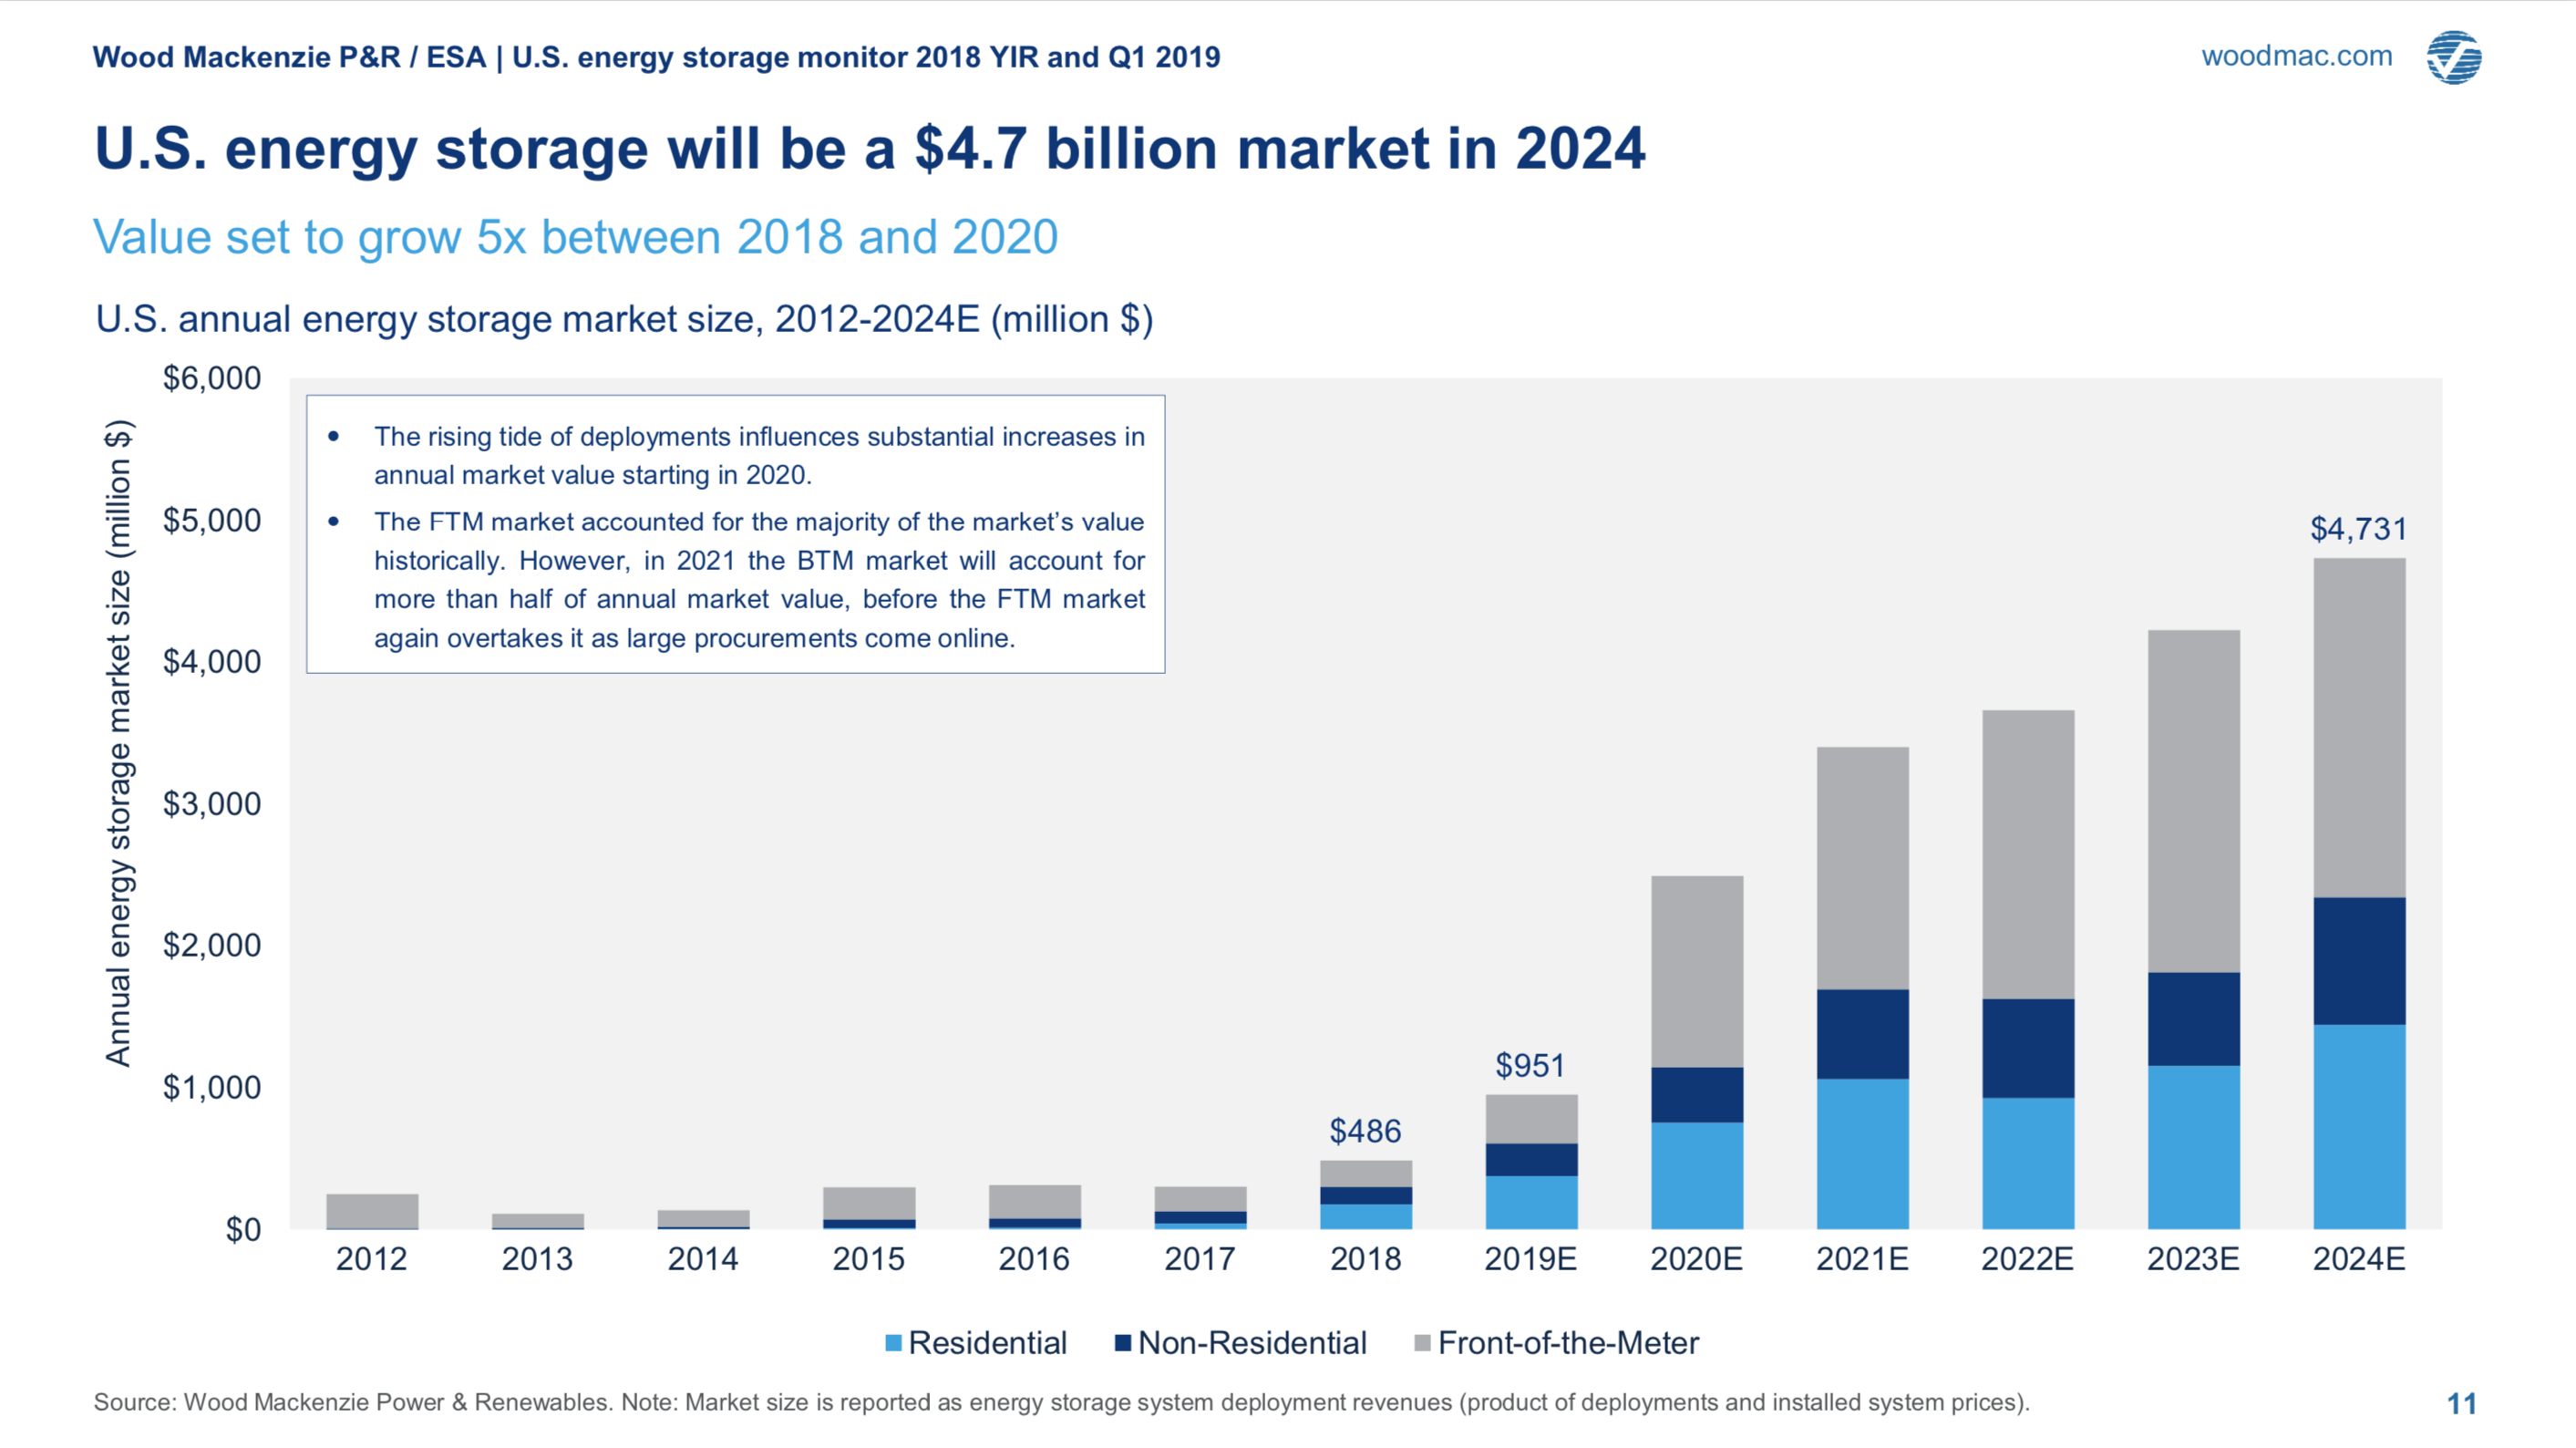
\includegraphics[width=1\textwidth]{US-ESM-2018-YIR-Executive-Summary-us-energy-storage-market-in-2024.png}
    \caption{Page from a 2018 Wood Mackenzie report \cite{USEnergyStorageMonitor2018YIRAndQ12019}}
\end{figure}
\FloatBarrier

The BloombergNEF (Bloomberg New Energy Finance) research team forecasts even larger energy storage growth in the coming decades. They project exponential growth from 9GW deployed as of 2018 to 1,095GW by 2040. In their words:

\begin{displayquote}
“This 122-fold boom of stationary energy storage over the next two decades will require \$662 billion of investment, according to BNEF estimates. It will be made possible by further sharp declines in the cost of lithium-ion batteries, on top of an 85\% reduction in the 2010-18 period.” \cite{EnergyStorageInvestmentsBoom}
\end{displayquote}

It should be noted that the BNEF report expects this growth to be filled largely with lithium-ion battery storage. But even if the cost of lithium-ion is cut in half, they will still be far more expensive than PHS. We will discuss these economics in more detail below.


\subsection{A Booming Energy Storage Market}
The nascent energy storage market looks poised for incredible growth. Public awareness is just beginning to spread through new high-profile initiatives. One such project is a \$3 billion pumped storage retrofit being planned for the Hoover Dam. According to the New York Times,

\begin{displayquote}
“Using Hoover Dam to help manage the electricity grid has been mentioned informally over the last 15 years. But no one pursued the idea seriously until about a year ago, as California began grappling with the need to better manage its soaring alternative-electricity production — part of weaning itself from coal-fired and nuclear power plants.” \cite{The3BillionPlanToTurnHooverDamIntoAGiantBattery}
\end{displayquote}

The Hoover Dam retrofit is a part of a larger boom in pumped hydro energy storage projects. In the next section we'll examine why pumped hydro could soon lead a surge of growth in the stored energy market.

\pagebreak[1]
\section{Why Pumped Hydro Energy Storage?}
As discussed above, 94\% of the world's energy storage capacity comes from pumped hydro storage. \cite{ElectricStorageCapacityInTheUnitedStates} Pumped hydro is affordable and effective with round-trip efficiencies sometimes exceeding 80\%. \cite{ESAPumpedHydroelectricStorage}

\begin{figure}[ht!]
    \centering
    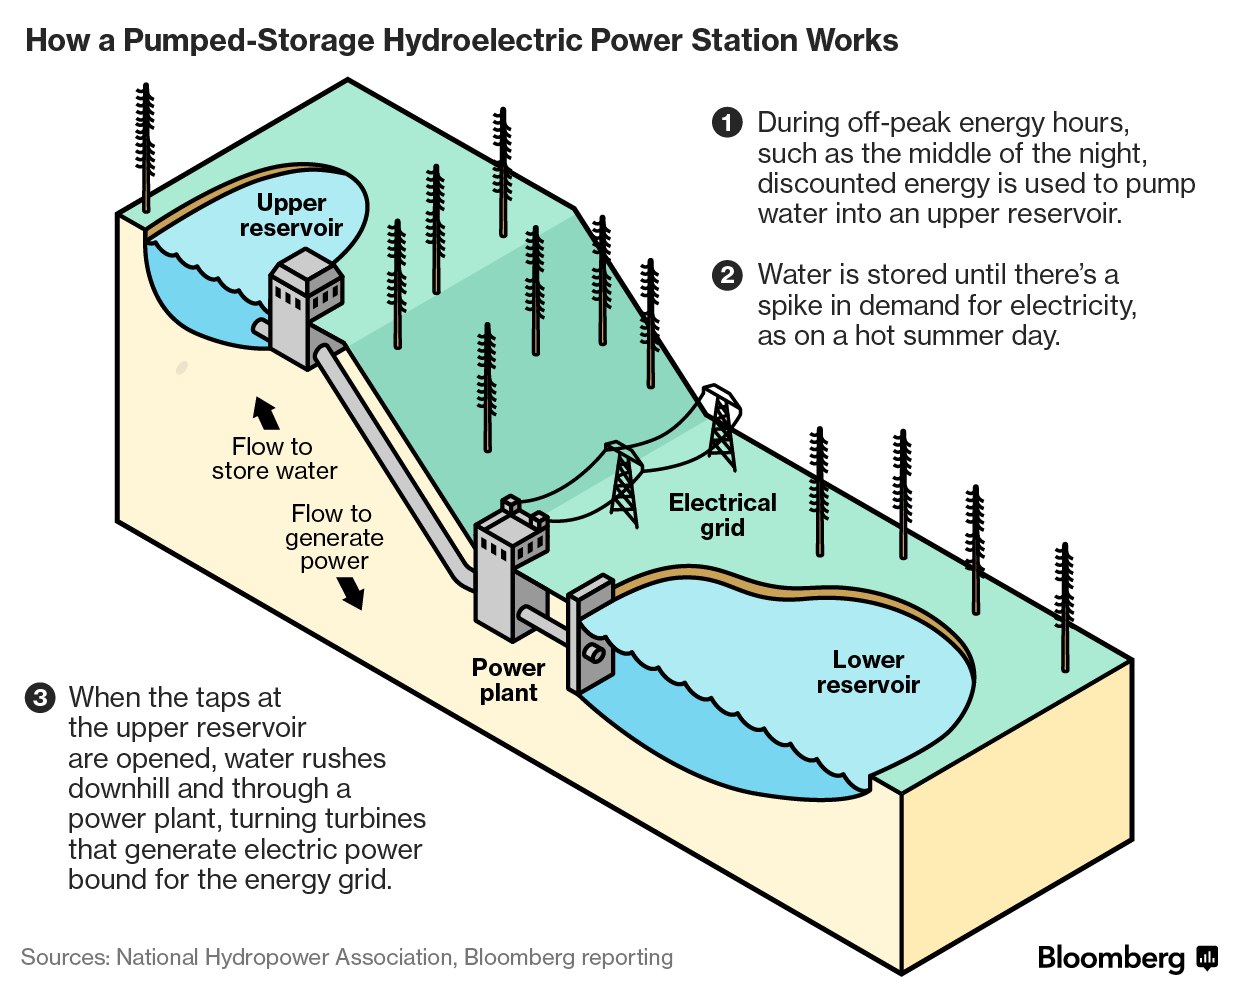
\includegraphics[width=1\textwidth]{bloomberg-how-pumped-storage-works.png}
    \caption{Graphic from Bloomberg \cite{QuestforBiggerBatteries}}
\end{figure}
\FloatBarrier

A Bloomberg article from 2018 called “The world's most beautiful Battery,” calls pumped hydro the “‘unsung hero’ of electricity storage solutions.” \cite{MostBeautifulBattery} The article details how pumped hydro plants were once a “little-seen corner of the electricity grid.” And now “they’re getting fresh attention across Europe and the U.S. as governments struggle to accommodate the surging supplies from wind and solar.” \cite{MostBeautifulBattery}

\subsection{The Clear Leader of Bulk Energy Storage}
Although there are many other kinds of energy storage deployed around the world \cite{OpenListOfNonPumpedStorageProjects}, and each of these are uniquely suited to specialized purposes, they are not used for bulk energy storage on a grid scale. Flywheels for example are “mainly used for power management rather than longer-term energy storage.” \cite{USGridEnergyStorageFactsheet}

A report from the University of Michigan, drawing on research from the U.S. DOE, offers a nice summary of Pumped Hydro's position amongst other alternatives.

\begin{figure}[ht!]
    \centering
    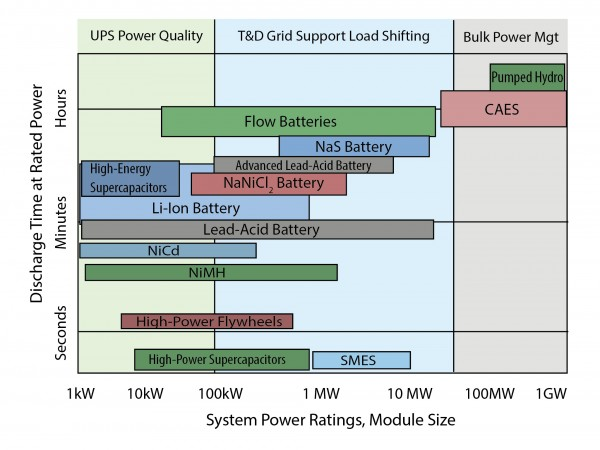
\includegraphics[width=.75\textwidth]{characteristics-of-energy-storage-technologies.jpg}
    \caption{Characteristics of energy storage technologies \cite{USGridEnergyStorageFactsheet}}
\end{figure}
\FloatBarrier

As shown in the figure above, there are only two proven technologies that work for Bulk Power Management. The only other solution besides PHS is one called CAES, or Compressed Air Storage.

\subsection{What About Compressed Air Storage?}
Compressed Air Storage (CAES) is indeed a feasible competitor to Pumped Hydro for delivering grid-scale bulk energy storage. However CAES has some disadvantages which disqualify it from being considered here. Most importantly CAES uses fossil fuels as a part of its process, so it's not carbon neutral. As explained by the NREL report mentioned above: “CAES technology is based on conventional gas turbine technology and uses the elastic potential energy of compressed air. Energy is stored by compressing air in an airtight underground storage cavern. To extract the stored energy, compressed air is drawn from the storage vessel, heated, and then expanded through a high-pressure turbine that captures some of the energy in the compressed air. The air is then mixed with fuel and combusted, with the exhaust expanded through a low-pressure gas turbine.” \cite{TheRoleOfEnergyStorageWithRenewableElectricityGeneration} Because CAES is not carbon neutral and requires an unusual site location, we will not consider it further. However, the NREL report does indicate that alternative designs may mitigate these limitations in the future. So perhaps CAES can be revisited in the future.

\subsection{What About Other Novel Solutions?}
There is always a chance that a young new technology will surprise the industry with rapid successful development. Here we examine some interesting but unproven ideas. Some of these may prove feasible for bulk energy storage in the coming years.

{\footnotesize
\begin{itemize}
    \item Advanced Rail Energy Storage: ARES is reported to provide long duration (8+ hours) of storage, round trip efficiency of over 80 percent, and levelized cost comparable to pumped storage. Its principal challenges have to do with price uncertainty and technology adoption. \cite{EnergyStorageCaliforniaClimateandEnergyGoals}

    \item Flow Batteries: Flow batteries store energy in electroactive solutions. Flow batteries offer advantages in terms of longer duration, longer cycle life, improved safety due to the non-flammable, non-toxic nature of the materials used, and potentially larger scale. Flow batteries, however, are still largely at the demonstration stage of technological development and prices remain high. \cite{EnergyStorageCaliforniaClimateandEnergyGoals}

    \item Sodium Sulfur Batteries: This technology is close to market. But reliability and safety issues remain a challenge. These concerns were highlighted when NGK Energy Storage’s sodium sulfur batteries caught fire in 2011. \cite{EnergyStorageCaliforniaClimateandEnergyGoals}

    \item Lead-acid batteries: Lead-acid batteries are slightly more expensive than sodium sulfur batteries, with higher life cycle cost. The main disadvantage of lead-acid is lower energy density and limited cycle life. \cite{EnergyStorageCaliforniaClimateandEnergyGoals}
\end{itemize}
}

While these ideas deserve research and attention, it would be dangerous to assume that unproven technologies like these may save us.
Considering our urgent need for additional energy storage, it is critical to acknowledge that pumped hydro is still our only proven source of zero-carbon bulk energy storage. Therefore, to minimize risk, we must rapidly develop more pumped hydro even as we explore alternative options.

\subsection{A PHS Case Study: The Kaprun Hydroelectric Station}
In “The world's most beautiful Battery” mentioned above, the article celebrates one particular hydro plant called the Kaprun hydroelectric station. Located high in the Austrian Alps, the Kaprun station offers a shining example of pumped hydro's success.

% \begin{figure}[ht!]
%     \centering
%     
\includegraphics[width=1\textwidth]{2018-kaprun-hydroelectric-station-battery-photo.jpg}
%     \caption{The Kaprun high mountain reservoirs. photographer: akos stiller/bloomberg \cite{MostBeautifulBattery}}
% \end{figure}
% \FloatBarrier

\begin{figure}[ht!]
    \centering
    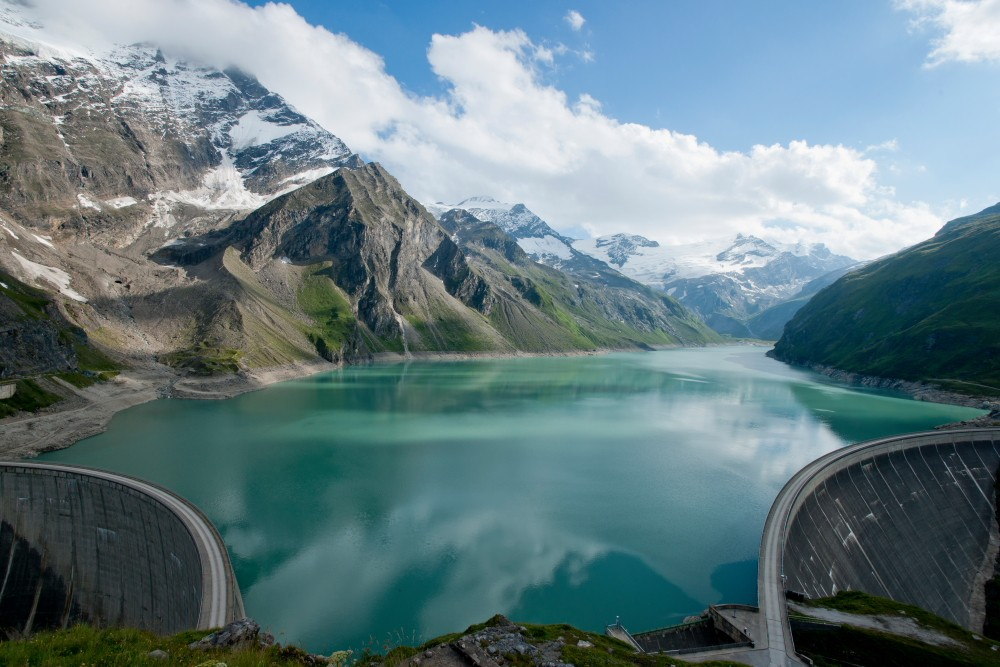
\includegraphics[width=1\textwidth]{kaprun-hydroelectric-station-photo.jpeg}
    \caption{A photo of the Kaprun high mountain reservoirs \cite{MostBeautifulBattery}}
\end{figure}
\FloatBarrier

At 70 years old, the Kaprun plant is still a valuable workhorse just as relevant in today's changing energy market. The plant boasts 830 megawatts of capacity, enough power to supply almost 100,000 households for more than a week. \cite{MostBeautifulBattery}

As demonstrated by Kaprun, pumped hydro storage technology is not only elegant and powerful, but also proven and durable. A similar plant built today would outlast a chemical battery plant many times over. Plants like Kaprun have inspired new growth in PHS. But the technology is now “at a tricky in-between stage,” says Jonas Rooze, a BloombergNEF analyst. \cite{MostBeautifulBattery} He believes the industry “will probably have to reinvent how they operate several times to capture value from the ever-evolving system.” \cite{MostBeautifulBattery} He says that “There’s capacity to build in Europe but right now it’s not in the money....For all of these projects you need a long-term vision.” \cite{MostBeautifulBattery} In other words, these large scale energy storage solutions still hold great promise, but only if we have the foresight to pledge large funds for long-term investments.

\subsection{A new Era for Pumped Hydro}
In a more recent Bloomberg article, journalist David R Baker makes a case that the time is indeed ripe for new long term visions to take on our newly evolving system. Baker identifies that “renewed interest is surging” in pumped storage technology. \cite{QuestforBiggerBatteries} According to the article, “The Federal Energy Regulatory Commission has issued 34 preliminary permits for companies and government agencies exploring projects in New York, Pennsylvania, Wyoming and elsewhere. Another 16 applications are pending.” \cite{QuestforBiggerBatteries}


\subsection{Pumped Hydro Pros and Cons}
Baker's article also offers succinct summaries of the pros and cons of pumped storage. Quoting Neena Kuzmich, a project manager for a proposed pumped storage facility near San Diego, Baker captures the sentiment behind this resurgence. In Kuzmich's words, “It’s not as glamorous as a battery. But it’s a tried and true technology that provides the volume that we need.” To illustrate the downside of pumped hydro, Baker cites BloombergNEF: “The projects can cost more than \$1 billion to build....Plus, securing permits, building dams and boring tunnels can take 10 years. And since the process often involves flooding valleys, most projects face resistance.” Baker reports that nine pumped hydro projects have been proposed in California. But even the project which is furthest along has met fierce opposition from environmentalists. Federal regulators approved the project in 2014 but construction has yet to begin. \cite{QuestforBiggerBatteries}

\subsection{Towards a long-term vision for Pumped Storage}
In section 2 we demonstrated that energy storage is critically important for decarbonizing our energy grid and curbing climate change. Section 3 has argued that pumped hydro is the best path forward for grid-scale investments in energy storage. In the following sections, we will make the case for a particular variation of pumped storage which could help bring the technology to market sooner. This variation takes the novel approach of replacing a lower reservoir with deep underground tunnels.

\pagebreak[1]
\section{Why Underground Pumped Hydro Energy Storage?}
Underground Pumped Hydro Energy Storage, or UPHS, is simply a pumped hydro solution which replaces the lower reservoir with an underground cavity mined from hard rock. This is not a new idea. Even though it has never been implemented on a large scale, the concept is well researched. In 1984, the Pacific Northwest Laboratory (sponsored by the US Department of Energy) authored a research paper called, “Underground Pumped Hydroelectric Storage.” The report (PNL report) concluded that “the UPHS concept is technically feasible and economically viable.” \cite{UndergroundPumpedHydroelectricStorage} It summarizes: “Underground pumped hydroelectric energy storage was conceived as a modification of surface pumped storage to eliminate dependence upon fortuitous topography, provide higher hydraulic heads, and reduce environmental concerns.” \cite{UndergroundPumpedHydroelectricStorage}

The PNL report analyzes the economic feasibility of the design concluding that, “A UPHS plant offers substantial savings in investment cost over coal-fired cycling plants and savings in system production costs over gas turbines.” \cite{UndergroundPumpedHydroelectricStorage} Regarding capacity potential it determines: “A UPHS plant would be in the range of 1000 to 3000 MW. This storage level is compatible with the load-leveling requirements of a greater metropolitan area with population of 1 million or more.” \cite{SubSurfacePumpedHydroelectricStorage}

These are striking conclusions. They make it clear that UPHS is, at the very least, a legitimate contender for our future's vast energy storage needs. And as such, this idea surely deserves further exploration. In the following section, we will examine past and `'current research on the technology.

\pagebreak[1]
\section{Underground Pumped Hydro Storage, Past Research}
In the 1984 PNL report mentioned above, the authors were optimistic about underground pumped hydro storage. The report concluded that, “while a project utilizing sub-surface reservoirs has yet to be completed, these types of projects are attractive due to their perceived site availability and their potential for reduced environmental impacts.” \cite{SubSurfacePumpedHydroelectricStorage} So, it may seem surprising that in the thirty-five years since the report, UPHS has never been developed. Why?

Although it's outside the scope of this report to analyze exactly why UPHS has not gained adoption, it is plausible that the reasons have not changed since the PNL report was published. As the report explained at the time, “Despite optimistic forecasts of technical and economic feasibility, so far no utility has committed funds to the design and construction of a UPHS plant....Even though UPHS has some environmental advantages over conventional pumped storage, higher cost remains an impediment to significant market penetration in the near future.” \cite{SubSurfacePumpedHydroelectricStorage}

The cost differences allude to were actually small, if even higher at all. The report notes that, “some feasibility studies” estimate capital cost to be “somewhat greater” than for conventional storage. \cite{SubSurfacePumpedHydroelectricStorage}). On the other hand, it noted a different study (the Charles T. Main Study) found that “Underground pumped hydroelectric storage compares favorably with conventional pumped storage” with costs being essentially the same. \cite{SubSurfacePumpedHydroelectricStorage}.


Still, the small difference, compounded with the risk of a new technology, must have been significant enough to deter interest. To this day, no major UPHS projects have been built. This was confirmed by at least one 2017 research paper which reported “no bibliographic evidence of UPSH plants constructed.” \cite{UndergroundPumpedStorageHydropowerPlantsUsingOpenPitMines}
But this could soon change as our current market conditions rapidly evolve.

\subsection{Past Research, Predicting Today's Market}
In the PNL report's closing section, the authors looked to the future, predicting which “changes in the electricity generating environment” would be necessary for the adoption of PHES. Here is the full list of changes which would be “likely to influence organizations toward UPHS commitments” \cite{SubSurfacePumpedHydroelectricStorage}:

{\footnotesize
\begin{enumerate}
    \item increase in the availability of capital and decreased interest rates
    \item increasing load growth within metropolitan areas
    \item trend toward joint ownership of large projects
    \item successful demonstration of advanced high-head reversible pump turbines
    \item full utilization of available and environmentally acceptable surface pumped hydro sites
    \item implementation of regulatory reforms to enable return on capital committed to construction of new facilities
    \item development of uniform institutional and legal procedures applicable to artificial surface and subsurface reservoirs
    \item demonstration of complete remote operability of the subterranean powerhouse in all modes of operation.
\end{enumerate}
}

Let's analyze and diagnose whether our current market has made such changes over the last few decades. For organization, we'll break this list into categories.

{\footnotesize
\begin{description}
    \item[Market demand: (see item 2 above)] Load growth has indeed increased since 1984. \cite{CenterForSustainableSystemsUniversityOfMichigan} But more importantly, a sharp increase in variable load is expected to accelerate market demand for energy storage.

    \item[Evolution of Research and Technology: (see 4 and 8)] Pumped Hydro technology has continued to advance in the last few decades. Research in advanced high-head turbines continues to increase load potentials. \cite{ParametricDesignOfAnUltrahighHeadPumpTurbine, 700m400MWClassUltrahighheadPumpTurbine} And where head height exceeds pump limitations, a multi-step approach can be used with intermediate reservoirs and powerhouses relieving head pressure from turbines below. \cite{SubSurfacePumpedHydroelectricStorage} Additionally, tunnel boring technology is faster and more efficient today which could significantly lower past cost estimates. \cite{VerticalConveyorsTheRobbinsCompany, TheBoringCompanyShowsOffItsFunctionalDemo}


    \item[Exhaustion of potential traditional Pumped Hydro: (5)] As discussed in the “Quest for Bigger Batteries” Bloomberg article, our current energy storage has already manifested a spike in pumped hydro permit applications. And many of these projects are stalled by fierce opposition driven by environmental concerns. So indeed, this fight over a shortage of feasible sites for traditional pumped storage has already begun. This problem will only get worse as the demand for energy storage grows year over year as projected. Under this shortage of traditional PHS sites, UPHS's environmental advantages could quickly justify slight additional upfront costs.

    \item[Regulation and Government Cooperation: (6 and 7)] Climate change has finally pressed governments and regulators to take urgent action. New York City and other governments have made bold commitments to mitigate risk through energy reform. Governments could soon view UPHS as a critical tool for attaining these goals. Especially within this political climate, regulators should be amenable towards such an environment-friendly technology.

    \item[Investor Interest: (1 and 3)] Although past research like the PNL report concluded that UPHS technology was “technically feasible and economically viable,” they understood that long construction time would challenge investors. The PNL report found that “Beyond the technical considerations...the quality of the bond market and availability of support through a utility consortium may ultimately determine economic practical capability.” In other words, it acknowledged that UPHS was just barely competitive with existing technologies. So due to long construction time and large upfront costs, UPHS was an infeasible investment for all but the largest of investors with the patience to leverage favorable loan conditions and industry cooperation. Until today, these conditions have been prohibitive for large-scale UPHS projects. But under today's rapidly changing political and energy market climates, the conditions could be ripe for this idea.
\end{description}
}

In conclusion, the energy market has indeed changed considerably since the PNL report was published in 1984. Technology has steadily evolved. The energy storage market is on the verge of exponential growth. Governments have promised energy market reform and have begun to inject capital into large-scale energy initiatives. These aligning factors could spin pumped hydro into a lucrative emerging market. With a convincing opportunity for long-term returns, UPHS could find an audience of patient investors with deep pockets.


\pagebreak[1]
\section{Underground Pumped Hydro, Current Research}
Considering that past research had already demonstrated the feasibility of underground pumped storage, the current state of UPHS research is disappointing. There are only a handful of small, experimental projects in development today which could be considered UPHS.

\subsection{Underground Gravity Storage With Heavy Piston Design}
One experimental design for underground energy storage involves a heavy “piston” of heavy rock mined from a vertical shaft. This design was once mentioned by science celebrity Bill Nye as an idea that he was “thoroughly charmed by” \cite{BillNyeBigThinkVideo} 6:50. The idea is developed by a company called Gravity Power. This piston concept is not really a UPHS design though. Because, while water is pumped into a drilled vertical shaft, the weight of water is not utilized to store energy. The water is pumped in a closed loop with water above and below the piston. The water really only serves to pressurize the shaft in order to lift the piston weight. In fact, the water's net weight is actually pumped in the opposite direction as the piston's weight, so it seems to actually detract from the efficiency of the system. \cite{GravityPowerNewTakeOnPumpedHydroEnergyStorage}

\begin{figure}[ht!]
    \centering
    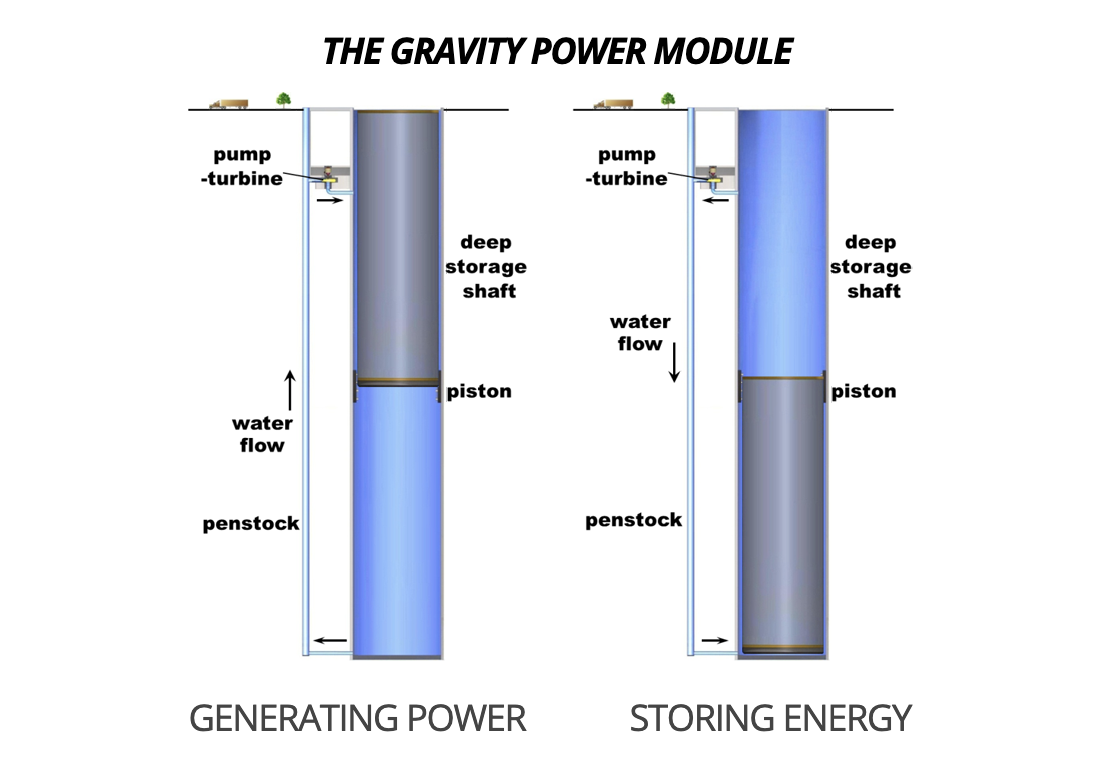
\includegraphics[width=1\textwidth]{gravity-power-diagram.png}
    \caption{Diagram of Gravity Power, LLC's scheme \cite{GravityPowerTechnologyPage}}
\end{figure}
\FloatBarrier

Our calculations raise doubt as to whether this design could be superior to underground pumped hydro. Because while the rock density might be about 2.5 times the density of water, the piston's bulk would restrict both its volume and the potential height it could travel, reducing its advantage. So it seems that this design would perform worse than UPHS, offering less storage capacity per meter of tunnel. (See Appendix: Calculations for Pumped Storage with Heavy Piston Design). We do concede however that this piston design eliminates the need for an upper reservoir. So perhaps the idea could still prove valuable for some locations where an upper reservoir is not possible.

\subsection{Underground Pumped Hydro in Abandoned Mines}
It seems that most UPHS projects in development today have set their sights on abandoned mines and rock quarries which offer an existing lower reservoir. There are multiple reports of such projects being researched and proposed, but it's unclear how many of these projects are actually getting completed. Some of these projects are:\cite{SubSurfacePumpedHydroelectricStorage, GermanCoalMineMayBePrimeForPumpedStorage, 250MWKidstonPumpedStorageHydroProject}
{\footnotesize
\begin{description}
    \item[1] The Elmhurst Quarry Pumped Storage Project (designed to be 50-250 MW)
    \item[2] The Riverbank Wisacasset Energy Center (1,000 MW)
    \item[3] The Prosper-Haniel coal mine in Germany (200 MW)
    \item[4] The Kidston Pumped Storage Hydro Project in Queensland, Australia (250 MW)
\end{description}
}

These projects slated for abandoned mines have smaller capacities, usually by an order of magnitude, than those suggested in the PNL report which proposed projects at about 3,000 MW with a 10 hour capacity. \cite{UndergroundPumpedHydroelectricStorage}

This report's authors were not able to determine how cost-competitive it would be to develop a bundle of smaller pit mine sites rather than developing one single centralized PHES site. But it does seem that there are ample mine sites around the world which would be suitable. There are about half a million abandoned mines in the United States. \cite{MappingInactiveMetalMinesAcrossTheUS} And according to hydroworld.com, there are thousands of abandoned rock quarries in the US National Park system alone. And these could be “converted into pumped storage facilities with less civil work than a greenfield development and minimal environmental impact.” \cite{PumpedStorageElmhurstQuarryProject} So it seems feasible that the supply of mines is plentiful. However, it's unclear what the average depths and volumes of these mines are as this report's authors have not yet been able to find a database that included those figures. It seems that a typical coal mine depth might be around 300-600m, \cite{UndergroundPumpedStorageHydroInAbandonedCoalMines} which is significantly less than the 1500m or greater depths proposed by the 1984 paper.


\subsection{UPHS Summary of Current Research}
In summary, there are no active research projects exploring grid-scale underground pumped storage as proposed in the 1984 PNL report. In the following section we'll argue that this is a missed opportunity, and that changing market conditions could make this technology more feasible and profitable than ever before.

\pagebreak[1]
\section{Why UPHS is Feasible Today}
As discussed above, underground pumped storage has been rigorously studied and generally determined to be “technically feasible and economically viable.” \cite{UndergroundPumpedHydroelectricStorage} To reach this conclusion, the PNL report drew on multiple case studies including, the Charles T. Main Study, the Argonne National Laboratory/Allis Chalmers Studies, the Potomac Electric Power Company Study, and the Commonwealth Edison/Harza Study. Citing the Charles T. Main Study, the PNL report states:

\begin{displayquote}
“Underground pumped hydroelectric storage compares favorably with conventional pumped storage. The construction costs were found to be essentially the same [i.e., in the range of \$300 to \$350/kW (1978 dollars)]. Operating and maintenance (O\&M) costs are essentially the same, possibly favoring UPHS.” \cite{UndergroundPumpedHydroelectricStorage}
\end{displayquote}

And further highlights some benefits of UPHS which could make it more advantageous than traditional pumped storage in some scenarios.

\begin{displayquote}
Underground pumped hydroelectric storage should appeal to a utility company in lieu of conventional pumped storage in that it minimizes site selection and acceptance problems; develops greater head and capacity; is more applicable in water-scarce areas; and lowers transmission costs and line losses by being located near load centers. \cite{UndergroundPumpedHydroelectricStorage}
\end{displayquote}


In spite of these advantages, no one has built any UPHS over the past few decades. It's possible that the idea was simply forgotten about and never considered until now. But as detailed above (see \textit{Past Research, Predicting Today's Market}), it's likely that sub optimal market conditions have kept the idea out of development. We believe that these conditions are recently turning in favor of UPHS.

\subsection{A Convergence of Favorable Factors for UPHS}
In the \textit{Past Research} sections above, we outlined the factors which were predicted “likely to influence organizations toward UPHS commitments.” These factors are much better aligned to favor UPHS today than they were in 1984.

As already mentioned, “renewed interest is surging” in traditional pumped hydro storage technology (see \textit{A new Era for Pumped Hydro} above). Developers are rushing to secure project permits in anticipation of parabolic growth in the energy storage market (see \textit{Wood Mackenzie} report above). However, this spiking demand faces resistance from an exhaustion of ideal sites and an increase in environmental concerns. These factors were cited by the PNL report as market drivers for UPHS.

Technological advances also favor UPHS. Tunnel boring technology and high-head turbine technology have evolved considerably. High-head turbine research has continued to optimize efficiency, though these gains are likely small. On the other hand, tunnel boring technology is poised for huge gains in efficiency, largely thanks to Elon Musk's \textit{The Boring Company}. According to Musk, the company's modified boring machine called Linestorm can dig 2-3 times faster than a conventional machine. And a radical new design called Prufrock will be expected to dig 10-15 times faster than the conventional competition.  \cite{TheBoringCompanyInformationSession} (video 52:03)

\begin{displayquote}
According to Elon Musk, Prufrock, the fully Boring Company designed machine will be, aspirationally, 15 times faster than current boring machines. Very likely 10 times faster.
\end{displayquote}

The new design is expected to parallelize basic functions, allowing for excavation, wall reinforcement, and earth removal to all be executed simultaneously. In Musk's own words, they intend to “automate segment direction,” incorporate a “passing lane” for incoming and outgoing materials, and implement a  “fast muck dump.” Of course some experts are skeptical about these unproven claims. \cite{ElonMuskTunnelingTechUnderLA} But if Musk is able to deliver on such speed improvements, it could drop digging costs by a factor of 10. This could in turn drastically reduce the cost of underground pumped storage since the cost is largely driven by tunneling costs. According to the PNL report, the lower reservoir of a UPHS plant likely represents about 30\% of the overall project cost.\cite{UndergroundPumpedHydroelectricStorage}

\subsection{Biggest Challenges for UPHS Today}
We presume that the largest obstacles facing UPHS developers today would be current unfavorable regulations, and any market aversion to long-term investments. Yet, both of these issues are steadily improving in today's political climate as governments and corporations rush to fulfill their decarbonization promises. The City of New York for example, is throwing real money behind these efforts. In their oneNYC report, they promise:

\begin{displayquote}
“We will continue to coordinate with public and private partners to create market opportunities for emerging technology and innovation, while helping to remove the technical, financial, and regulatory barriers that limit scale.” \cite{OneNYC2050FullReport} -- New York City
\end{displayquote}

And New York State has sponsored a financial entity called NY Green Bank to accelerate clean energy deployment. From the Green Bank website, “NY Green Bank is a State-sponsored, specialized financial entity working with the private sector to increase investments into New York’s clean energy markets, creating a more efficient, reliable and sustainable energy system.” \cite{NYGreenBank} According to the Coalition for Green Capital, in June 2017 the New York Green Bank became profitable after just a few years of operation. They had made investments of \$409.4 million to support projects with a total cost of between \$1.2 and \$1.4 billion. \cite{NYGreenBankPathToProfitability}

\begin{figure}[ht!]
    \centering
    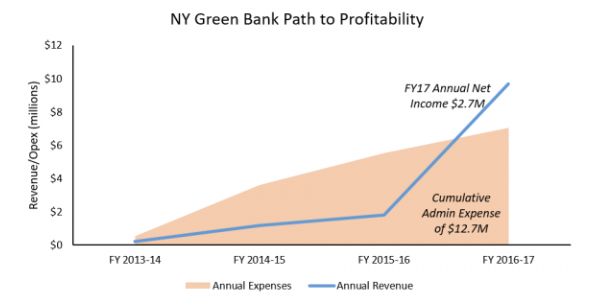
\includegraphics[width=1\textwidth]{new-york-green-bank-path-to-profitability.png}
    \caption{The New York Green Bank became profitable in 2017 just a few years after its launch. \cite{NYGreenBankPathToProfitability}}
\end{figure}
\FloatBarrier

\pagebreak[1]
\section{UPHS Case Study Technical Specifications}

\begin{figure}[ht!]
    \centering
    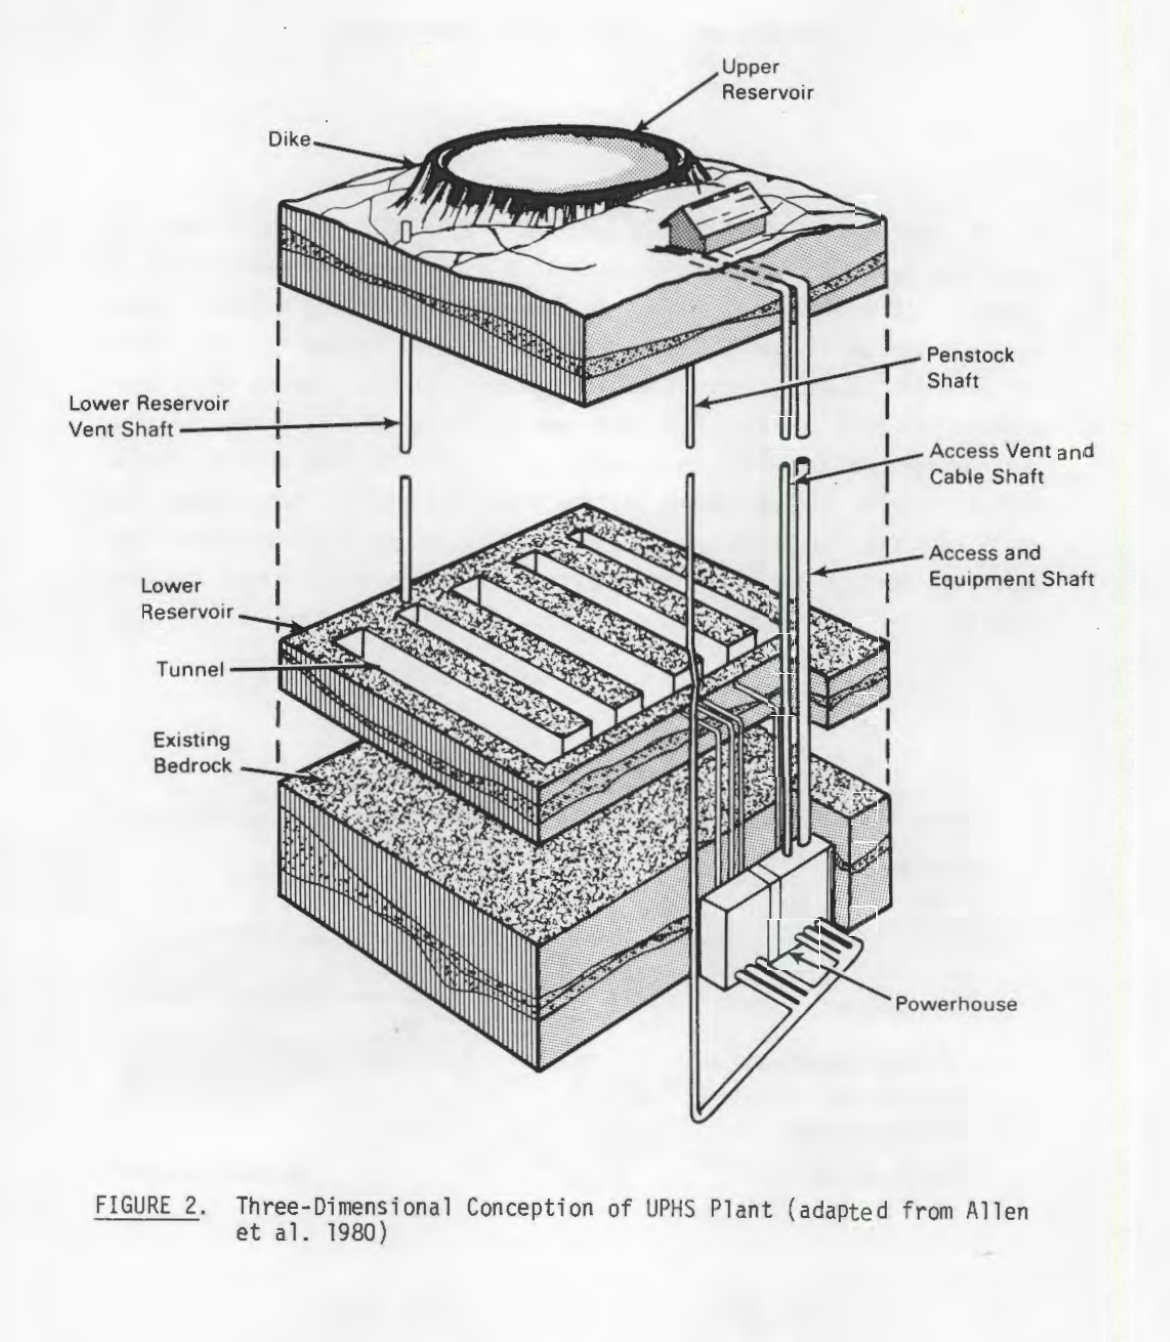
\includegraphics[width=.75\textwidth]{pnl-report-diagram-2.png}
    \caption{Image from the Pacific Northwest Laboratory Report: Three-Dimensional Conception of UPHS Plant (adapted from Allen et al. 1980) \cite{UndergroundPumpedHydroelectricStorage}}
\end{figure}
\FloatBarrier

The PNL report cites the Potomac Electric Power Company Study as
“without a doubt, the definitive design study for UPHS,” which it says, “will provide the baseline against which all UPHS development in the future will be referenced.” This study (PEPC study) which was also sponsored by the US Department of Energy, provides detailed technical designs.

The study conducted cost comparisons of various configurations for a 2000-MW plant. And it concluded that a two-step multi-pump design was optimal because it optimized head height and therefore minimized the volume of lower reservoir excavation. \cite{UndergroundPumpedHydroelectricStorage}

\subsection{PEPC Study: Two-Step Design with Reversible Pump-turbines}
The PEPC study's optimized design called for single-stage reversible pump-turbines with identical layout and design. Each step consisted of three pump-turbine/motor-generator sets, each of 333-MW rating and each operating at 720 rpm under a nominal head of 762 m (2500 ft). With two steps combined, the overall nominal head was 1525 m (5000 ft). The study acknowledges that future technological development could significantly raise the head height or achieve the same head height in only one step.

\subsection{PEPC Study: General Architecture}
In addition to the main vertical penstock shaft, four
other shafts were planned, ranging in depth from 1525 to 1677 m (5000
to 5500 ft). Three of these shafts were to contain hoisting conveyances for main power transmission, and control cables. The fourth, an air vent shaft, was to allow atmospheric air admission to and from the lower and intermediate reservoirs.

Construction of all shafts was to be accomplished by sinking from the surface using conventional drilling and blasting methods.

\begin{figure}[ht!]
    \centering
    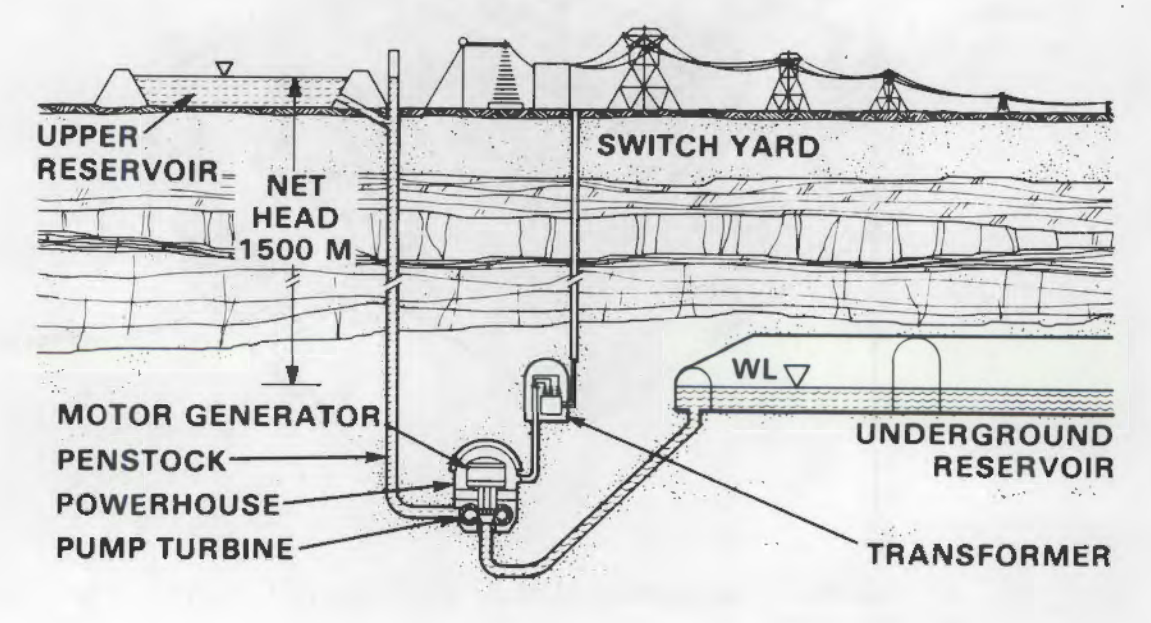
\includegraphics[width=.75\textwidth]{pnl-report-diagram-1.png}
    \caption{Image from the Pacific Northwest Laboratory Report: Cross Section of UPHS plant \cite{UndergroundPumpedHydroelectricStorage}}
\end{figure}
\FloatBarrier

\subsection{PEPC Study: Penstock Specifications}
The vertical penstocks were to have diameters of 5.8 m (19ft) and be designed for a maximum flow of 153 ($m^3$/sec) (5400 cfs).

The penstock walls were to have rock bolt support and a permanent concrete lining provided with a drainage system. The penstocks were to turn to the horizontal at the powerhouse levels, and concrete-lined manifolds were to form three 3.35-m (11-ft) diameter penstocks at each level. An 88-m (290-ft) length of the penstocks upstream from the powerhouses were to be lined with 7-cm (2 3/4-in.) thick high-strength steel lines that have flanged connection penstock valves upstream of the pump-turbine spiral cases.

\subsection{PEPC Study: Excavated Tunnel Specifications}
The PEPC study's excavation plan included 12 tunnels of substantial cross section, 26 x 20 m ( 85 x 65 ft), interconnected by smaller air and water collector tunnels at the extreme ends of the reservoir system.

The excavation volume was to be 6,012,900 $m^3$ (7,860,000 $yd^3$), which included 2.3\% for “safety” storage to prevent overfilling of the lower reservoir, and a further 0.3\% for freeboard. The main tunnels in the lower reservoir were to be oriented with their axes approximately perpendicular to the strike of the rock foliation in order to provide more desirable conditions for rock support of the larger spans. All of the storage caverns within the lower reservoir were to have curved side walls to reduce tensile stress zones. They were to be constructed at grades allowing free drainage upon dewatering. Provision was allowed for isolation of any one third of the reservoir with “stoplogs” to permit reservoir cavern inspection without disrupting plant operation.

\pagebreak[1]
\section{UPHS Site Selection Considerations}
The geology of the United States is sufficiently well known to determine areas of favorable development for UPHS. Site exploration can be aided from existent databases and interactive maps.

\subsection{UPHS Site Selection: Geology}
According to the PNL report, the lower reservoir of a UPHS system must be mined from rock which is essentially impervious. Pervious water-bearing sandstones, such as the artesian Dakota formation of the Great Plains, are not suitable for UPHS. Almost all other rocks are so dense as to be impervious for all practical purposes. \cite{UndergroundPumpedHydroelectricStorage}

\begin{figure}[ht!]
    \centering
    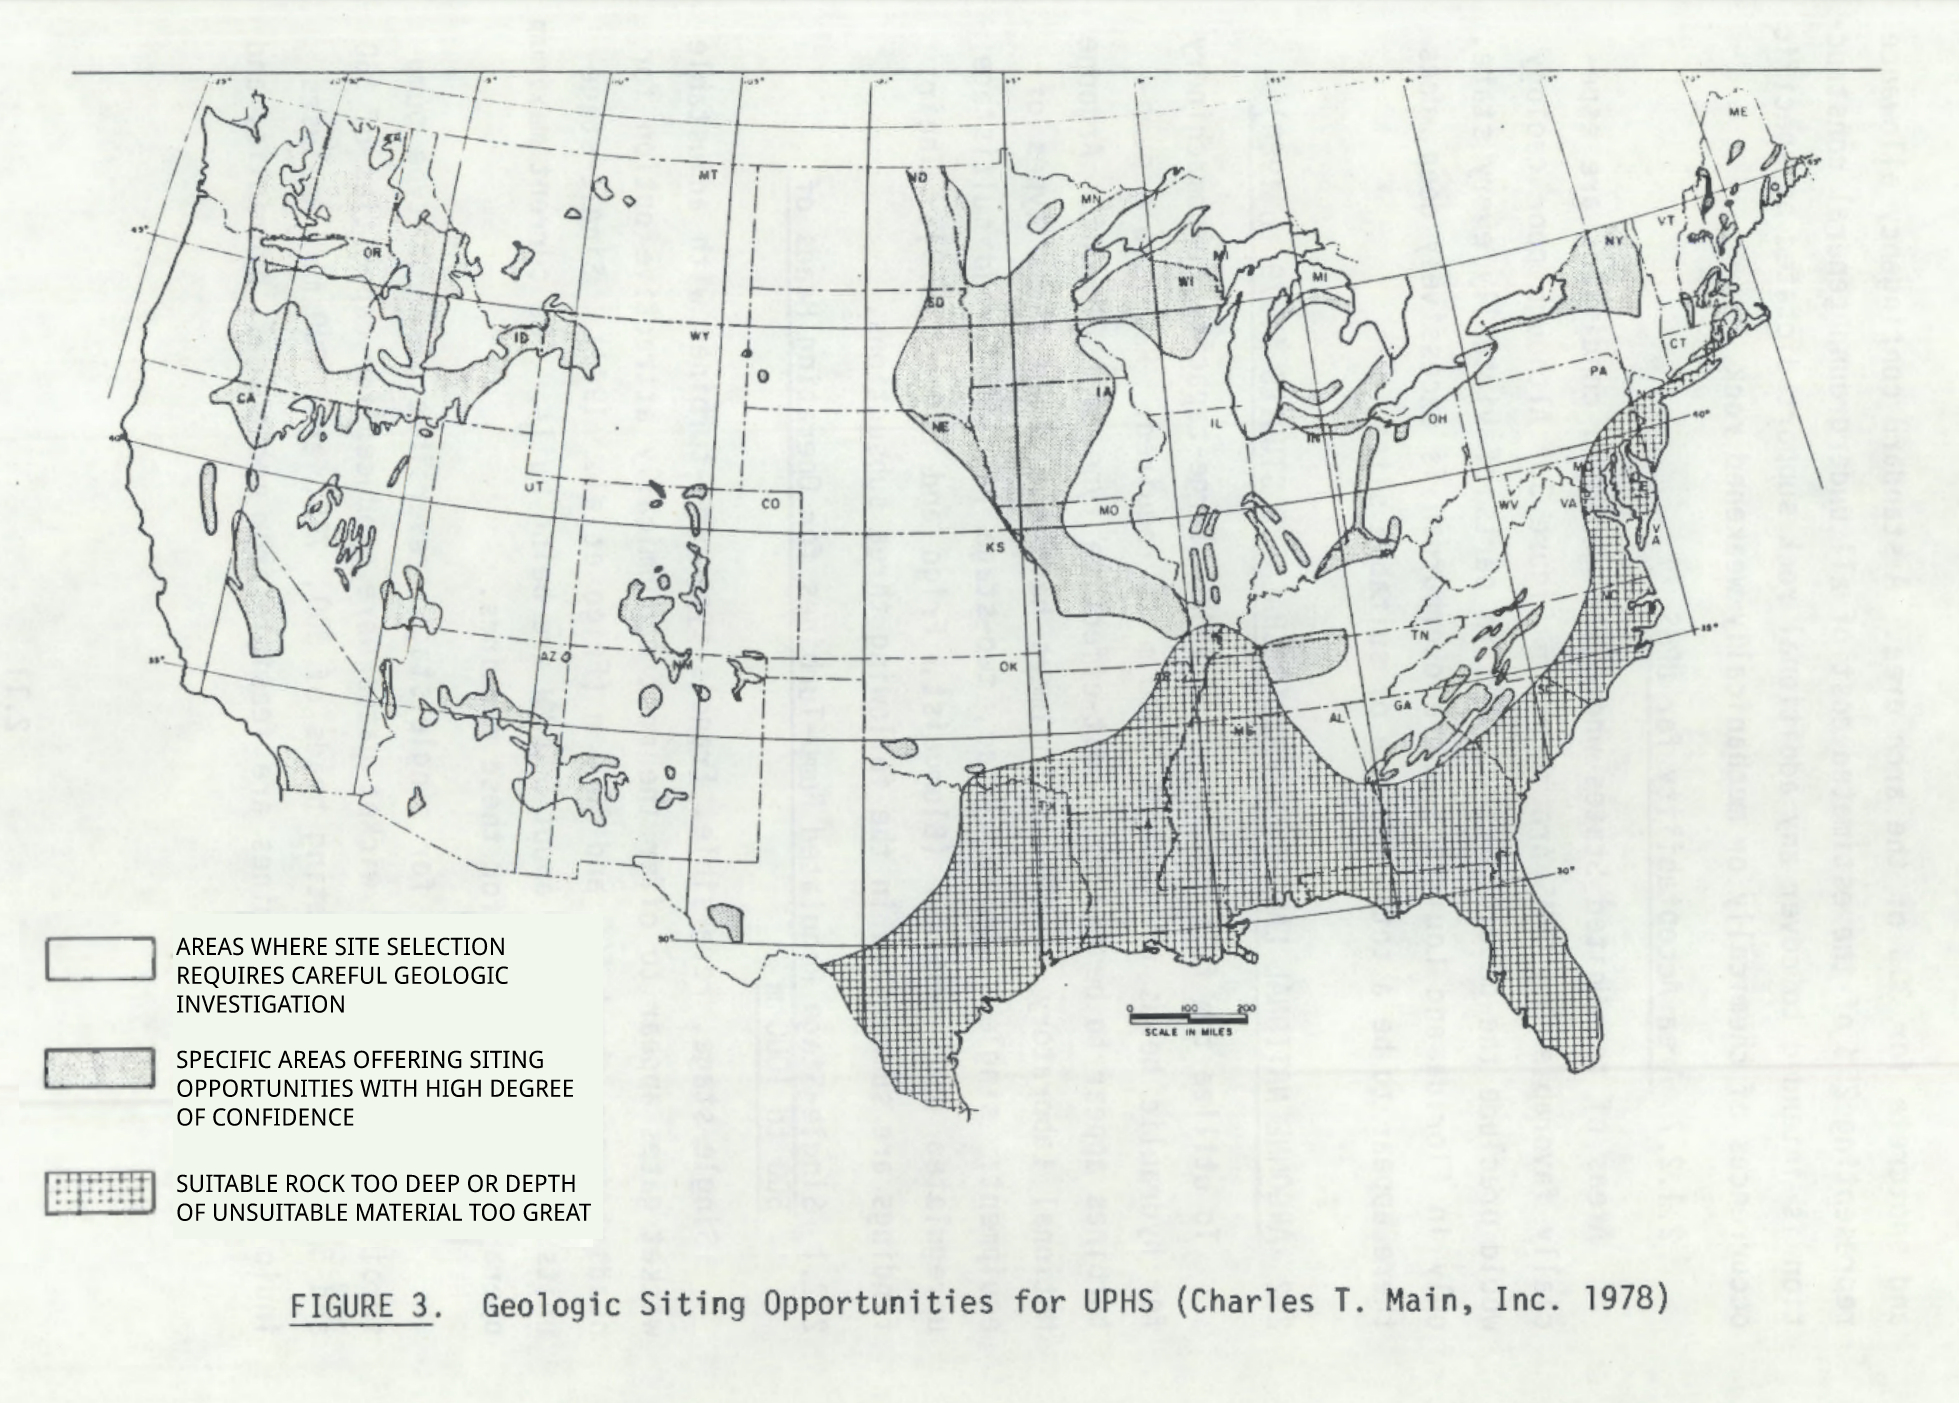
\includegraphics[width=1\textwidth]{pnl-report-geologic-siting-opportunities-for-uphs-text-overlay.jpg}
    \caption{Image from the Pacific Northwest Laboratory Report: suitable U.S. locations for UPHS (text enlarged). \cite{UndergroundPumpedHydroelectricStorage}}
\end{figure}
\FloatBarrier

As shown in the map above, most States in the US have at least some suitable areas for UPHS. Most areas require bore hole sampling to verify a site's geology down to the required depths.

For closer inspection of sites which are likely to be suitable, a detailed geologic map may be consulted.

\begin{figure}[ht!]
    \centering
    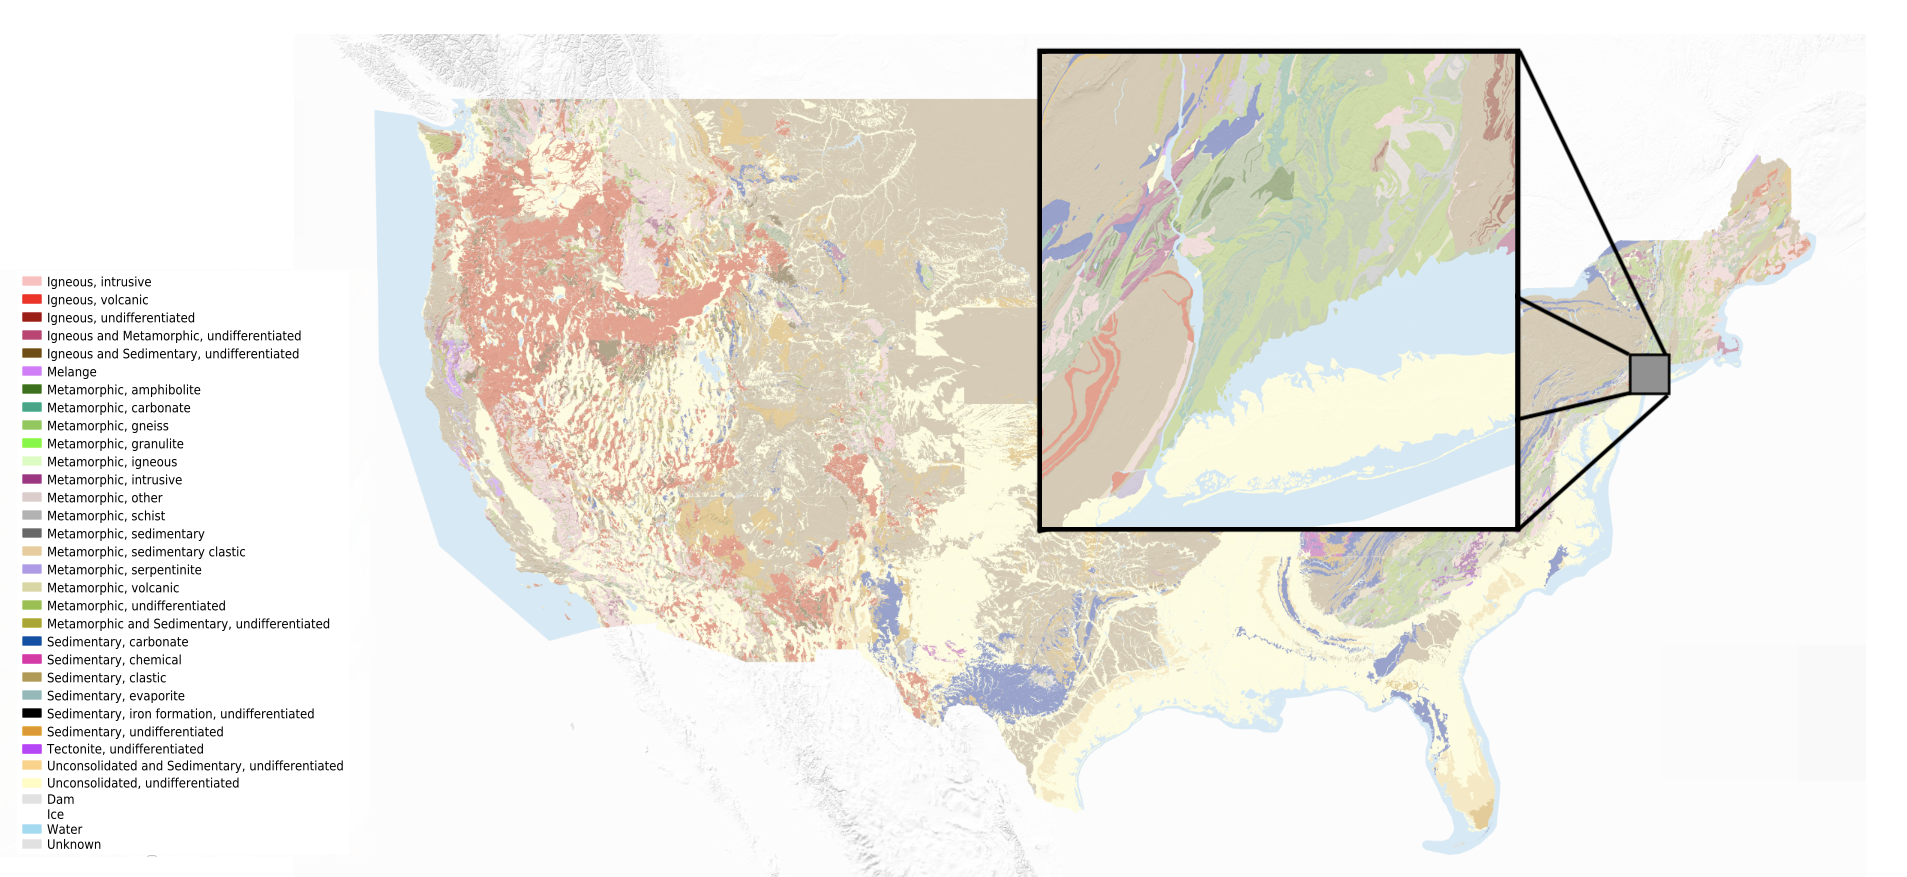
\includegraphics[width=1\textwidth]{usgs-gov-map-of-new-york-city-area.png}
    \caption{Geologic map of the U.S. with a close up of the NYC area -- usgs.gov \cite{MineralResourcesOnlineSpatialDataGeologicmaps}}
\end{figure}
\FloatBarrier

In the geologic map above, the New York City Area is shown to have a diverse mix of geology just north of the city which should include suitable sites for UPHS.

\subsection{UPHS Site Selection: GIS Analysis of Water and Elevation}
The Australian National University has recently compiled an amazing database and interactive map based on their research of potential sites for pumped hydro energy storage (PHS, also known as PHES). They found these sites using GIS algorithms. Based on factors like elevation, proximity, area, and volume, they calculated hypothetical pairs of upper and lower regions considering both existing dams and potential dammable areas. In their words:

\begin{displayquote}
“We found about 616,000 potentially feasible PHES sites with storage potential of about 23 million Gigawatt-hours (GWh) by using geographic information system (GIS) analysis. This is about one hundred times greater than required to support a 100\% global renewable electricity system.”
\end{displayquote}

\begin{figure}[ht!]
    \centering
    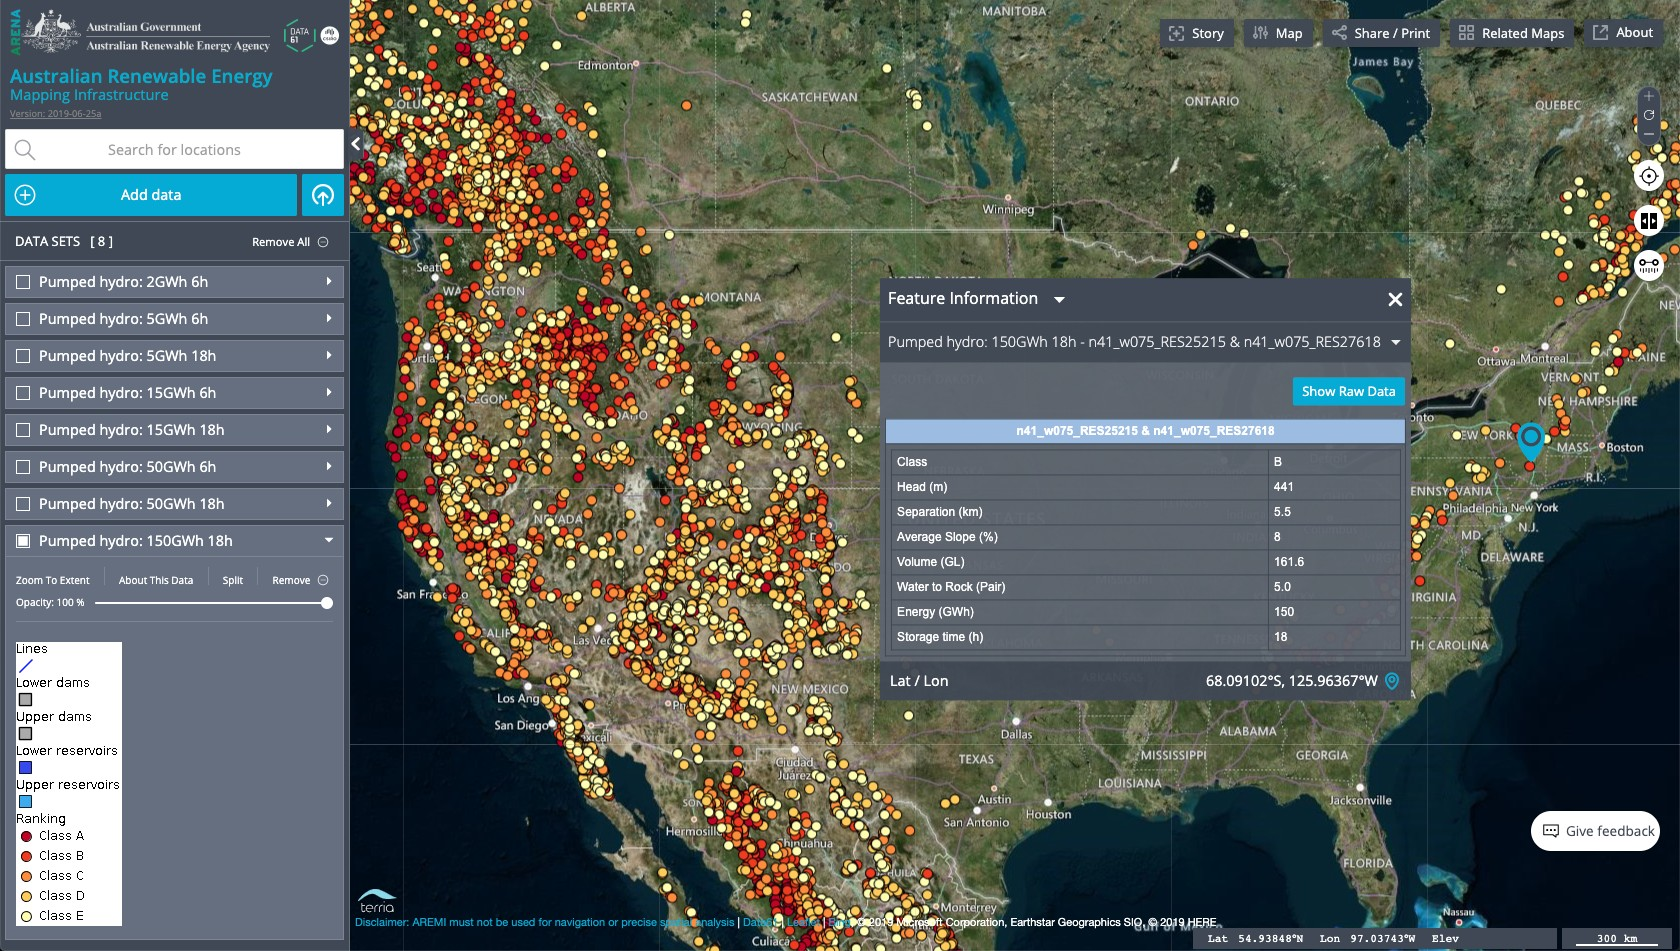
\includegraphics[width=1\textwidth]{australian-national-university-global-phes-atlas.jpg}
    \caption{Australian National University PHES Atlas - global search tool" \cite{AustralianNationalUniversityGlobalPHESAtlas}}
\end{figure}
\FloatBarrier

This map only considers sites for traditional PHS, not UPHS. But it can of course also aid in the research of potential sites for underground pumped hydro. This is especially true because the most optimal UPHS sites will likely make use of an existing dam or PHS site.

\begin{figure}[ht!]
    \centering
    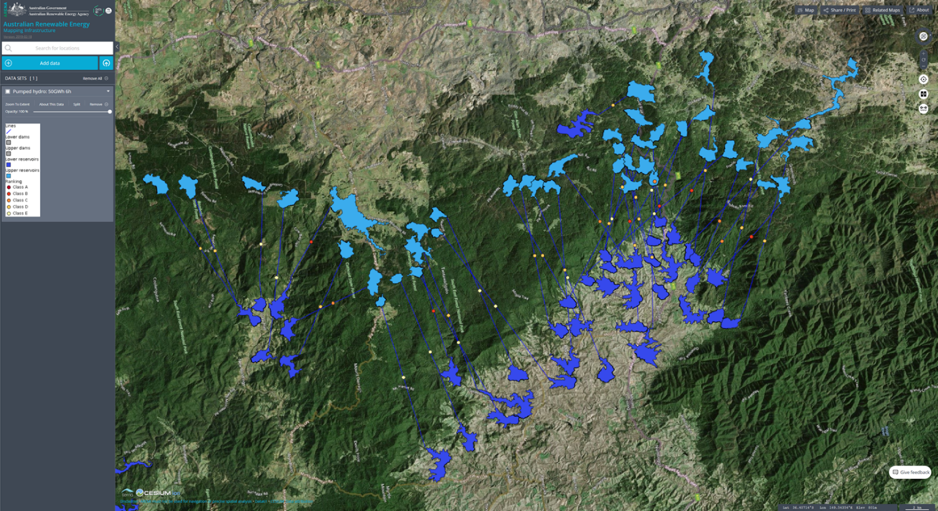
\includegraphics[width=1\textwidth]{australian-national-university-global-phes-atlas-water-overlay.png}
    \caption{Australian National University PHES Atlas - hypothetical PHS site overlay layer" \cite{AustralianNationalUniversityGlobalPHESAtlas}}
\end{figure}
\FloatBarrier

\subsection{UPHS Site Selection: Consideration of Sea Water Usage}
Sea water pumped storage is a very interesting modified form of pumped storage which uses the ocean as one of its reservoirs. The first project to successful employ this design was the Okinawa Yanbaru Seawater Pumped Storage Power Station in Japan. \cite{SeaWaterPumpedStoragePowerPlant}

\begin{figure}[ht!]
    \centering
    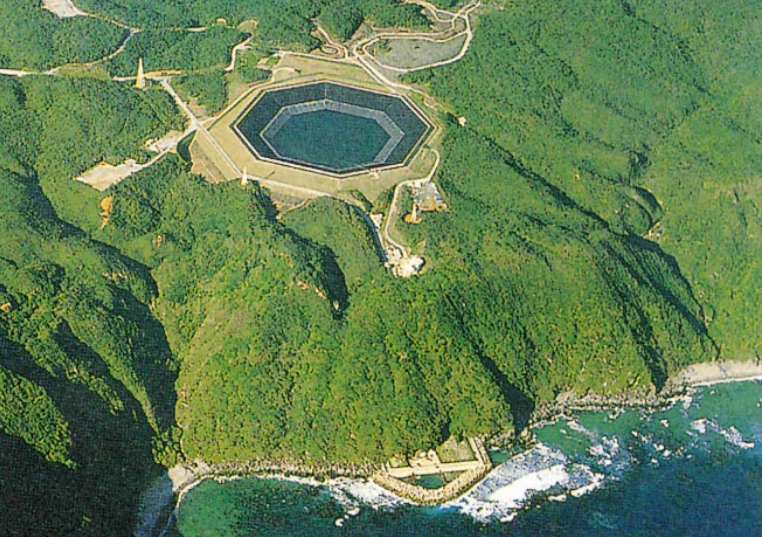
\includegraphics[width=.75\textwidth]{kaprun-hydroelectric-station.png}
    \caption{Birds eye view of the Okinawa Yanbaru Seawater Pumped Storage Power Station in Japan \cite{DevelopmentOfPumpTurbineForSeawaterPumpedStorage}}
\end{figure}

The Okinawa station was built in 1999 by the Japanese Ministry of Economy, Trade and Industry. It operated until 2016 when it was shut down because the demand for electric power in Okinawa had not grown as predicted. \cite{ExperimentalPowerPlantInKunigamiDismantled}

The Okinawa plant had 30 MW of storage. The lower reservoir was the Philippine Sea. The water was pumped 136 m up to an artificially excavated octagonal reservoir. Because sea water is highly corrosive, the
penstock and tailrace were constructed with fibre-reinforced plastic instead of steel, and the surface of the upper reservoir was covered with an impermeable liner to prevent seawater from leaking and damaging the surrounding vegetation. The pump turbine was partially made of seawater-resistant stainless steel. \cite{SeaWaterPumpedStoragePowerPlant} The outlet of the tailrace was  surrounded by tetra-pods for protection from waves. \cite{DevelopmentOfPumpTurbineForSeawaterPumpedStorage} Further research on the sea water pumped storage discusses other important factors such as preventing barnacle adhesion from reducing pump efficiency. \cite{DevelopmentOfPumpTurbineForSeawaterPumpedStorage}


\pagebreak[1]
\section{UPHS: New Innovations and Hybrid Designs}
In this section we will propose various innovations and hybrid designs based on existing technologies which could further enhance the efficiency of underground pumped hydro energy storage.

...\textit{* Redacted *}

UPHS could also be used to augment the capacity of existing traditional PHS sites. The UPHS plant could be installed beside the lower reservoir to effectively raise the head of the combined system and increase the overall potential storage capacity.

...\textit{* Redacted *}

The PHES Atlas project mentioned above has said that future versions of their study will include brownfield sites (existing reservoirs, old mining sites). It's feasible that these brownfield sites could be used as either upper or lower reservoirs for potential PHES sties.

\textit{* Redacted remainder of section. For further information and partnership opportunities, contact Eric Chaves at syllablehq.com.}

\pagebreak[1]
\section{UPHS: Optimized Site Selection}

\textit{* Redacted. For further information and partnership opportunities, contact Eric Chaves at syllablehq.com.}


\pagebreak[1]
\section{UPHS: Estimated Costs and ROI}
This section discusses the estimated costs of underground pumped hydro energy storage. It cites current research validating some of the figures from the PNL report on which we have drawn heavily.

\subsection{UPHS Construction Cost (Installed Cost)}

According to the PNL report, the total direct cost of a UPHS plant built in 1983 would be estimated at $\$500 * 10^6$ for a 1000-MW plant in 1983 dollars.\cite{UndergroundPumpedHydroelectricStorage} (about \$1.3 Billion in today's dollars. \cite{CPIInflationCalculator}). Note that this works out to \$1,300/kW.

As cited above, this cost compares favorably with conventional pumped storage. (\$300-\$350/kW in \$1978 \cite{UndergroundPumpedHydroelectricStorage}, which is about \$1,180-\$1,375/kW \$2019 \cite{CPIInflationCalculator}).

We can cross reference these numbers with more recent studies. According to a 2012 report by the International Renewable Energy Agency (2012 IRENA report), the installed costs for Large Hydro Plants were as low as \$1,050/kW (\$1,176/kW in \$2019). The costs were as high as \$7,650/kW (\$8,568 in \$2019) \cite{RenewableEnergyTechnologiesCostAnalysisSeries}. This large range is partly due to outliers with very large cost overruns. For our purposes of validating prices from the PNL report, we will just note that the low end construction cost for contemporary PHS (\$1,176/kW) is indeed comparable to the PNL report's low end construction cost for UPHS (\$1,180/kW).

\subsection{UPHS Operations and Maintenance (O\&M) Costs}
As cited above, the PNL report estimated that operating and maintenance (O\&M) costs for UPHS should be essentially the same as traditional pumped storage, possibly favoring UPHS. \cite{UndergroundPumpedHydroelectricStorage} According to the 2012 IRENA report, the yearly operations and maintenance costs for PHS are about 2 – 2.5\% of the installed cost.

\subsection{UPHS Levelized Cost of Renewables Combined with Energy Storage}
In a recent study published by MIT, researchers analyze profiles of energy storage which would be needed for low-carbon energy sources like wind and solar to meet grid demand in a cost-competitive market.

The study (MIT study) samples four locations in the United States in order to represent a diversity of potential energy capacity profiles for solar and wind across the country. The study determined that energy storage capacity costs would need to fall to \$20/kWh in order to allow a wind-solar mix to provide baseload electricity at competitive costs with existing power plants.

In order to account for the unique inter- and intra-year energy resource variations, the calculations considered 20 years of solar and wind fluctuations for each area. To compare the real costs of each technology, the study calculates the levelized cost of shaped electricity (LCOSE). Shaped electricity cost refers to the price of electricity bundled into contracts and priced for specific locations and times. The levelized cost refers to the minimum constant price of electricity which would be required over the lifetime of a plant in order to cover its costs.

The study considers two different classes of energy storage which it denotes as Tech I and Tech II. Tech I consists of cost efficient technologies like pumped hydroelectric storage (PHS), compressed air energy storage (CAES), and proposed flow battery technologies using highly abundant and low-cost elemental constituents. Tech II consists of future Li-ion batteries after further cost reduction, and possibly other closed battery technologies, flywheels, and supercapacitors. \cite{StorageRequirementsAndCostsOfShapingRenewableEnergy}

The study calculates various market scenarios in which a cost-optimal mix of wind, solar, and energy storage would reach costcompetitiveness with various existing energy sources.

The following list shows various Tech I energy storage price points which could pair with wind and solar in order to undercut corresponding current technologies.
{\footnotesize
\begin{enumerate}
    \item At \$10-20/kWh energy storage: nuclear fission baseload electricity (\$0.075/kWh)
    \item At \$5/kWh energy storage: peaker natural gas plant (\$0.077/kWh)
    \item At \$30–70/kWh energy storage: generic baseload (\$0.10/kWh)
    \item At \$30–90/kWh energy storage: generic intermediate (\$0.10/kWh)
    \item At \$10–30/kWh energy storage: generic bipeaker (\$0.10/kWh)
    \item At \$10–30/kWh energy storage: generic peaker electricity (\$0.10/kWh)
\end{enumerate}
}

The study concludes that Tech I energy storage could hit these rates (e.g. PHS), but Tech II storage could not (e.g. Li-ion chemical batteries)

The study then acknowledges however that Tech II battery storage could still be a compatible option for wind+solar+storage mixes, but not without giving up 100\% availability. This is because of the increasingly high costs of energy storage (diminishing returns of investment) as availability requirements approach 100\%.

\begin{figure}[ht!]
    \centering
    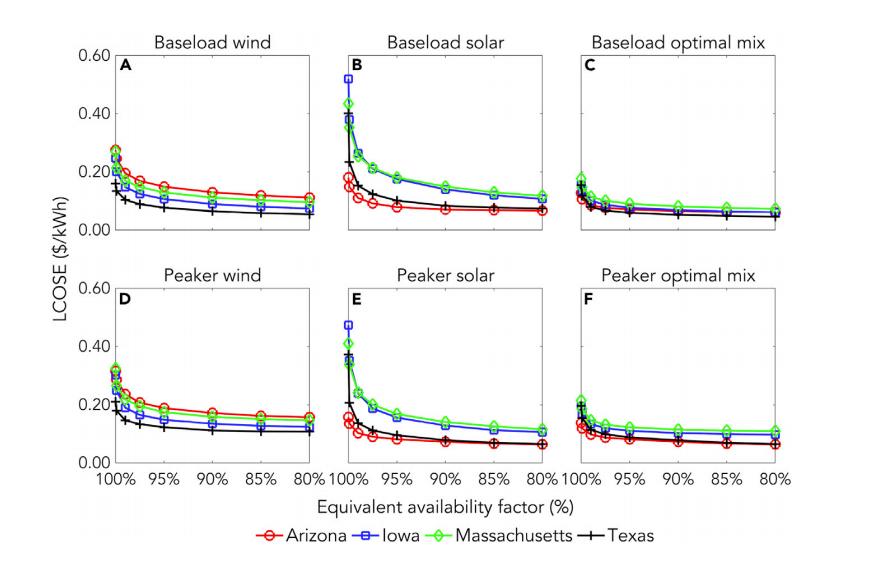
\includegraphics[width=1\textwidth]{cost-as-function-of-availability-factor.png}
    \caption{Electricity Cost Dependence on Equivalent Availability Factor for Tech II -- \cite{StorageRequirementsAndCostsOfShapingRenewableEnergy}}
\end{figure}
\FloatBarrier

As shown in the charts above, the energy storage cost rate of change is steep close to 100\% EAF (equivalent availability factor), but then it levels out. As the MIT study explains, these charts illustrate how an availability reduction of just 5\%, can drastically reduce energy prices and raise our energy capacity cost target from \$20/kWh to \$150/kWh.

At \$150/kWh, Tech II storage solutions like Li-ion chemical batteries could be feasible for some regions. This would of course require some other energy solution to provide availability for the remaining 5\% of the time which is a non-trivial problem to solve.

\subsection{UPHS: Estimated Levelized Cost of Energy}
The levelized cost of a power plant is the minimum constant price of electricity required over the lifetime of a plant in order to cover its costs. As discussed above, both the construction costs and O\&M costs of a UPHS plant are comparable to a traditional PHS plant. The 2012 IRENA report determines that the levelized power cost of a typical large hydro plant is about \$0.02–\$0.19/kWh in \$2010 (\$0.02–\$0.22/kWh in \$2019). This calculation assumes a 10\% cost of capital.

These numbers align with a more recent IRENA report outlining Renewable Power Generation Costs in 2017 (2017 IRENA report). This report shows that the global weighted average levelized cost of electricity from new hydropower projects in 2017 was US\$0.05/kWh. This was lower than any other power source that year. \cite{RenewablePowerGenerationCostsIn2017}

\begin{figure}[ht!]
    \centering
    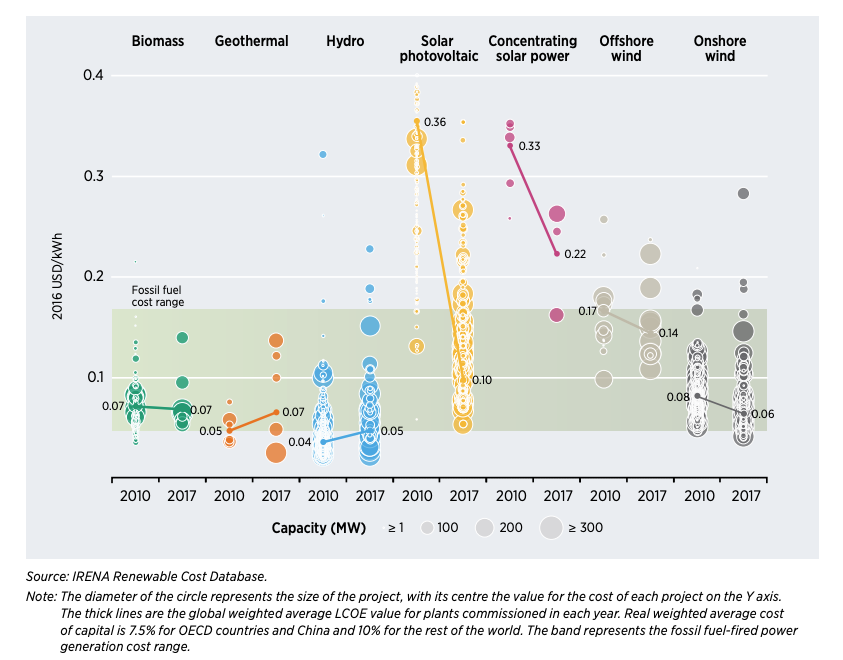
\includegraphics[width=1\textwidth]{renewable-power-generation-costs-in-2017.png}
    \caption{From IRENA: Global Levelized Cost of Electricity from Utility-Scale Renewable Power Generation Technologies, 2010-2017 (2016 \$/MWh) \cite{RenewablePowerGenerationCostsIn2017}}
\end{figure}
\FloatBarrier

We can calculate an estimated Levelized Cost of Energy Estimations using a simplified formula.

\begin{displayquote}
sLCOE = (overnight capital cost * capital recovery factor + fixed O\&M cost) / ((24*365) * capacity factor) \cite{SimpleLevelizedCostOfEnergyCalculator}
\end{displayquote}

The \textit{overnight capital cost} is the initial construction costs. The \textit{capital recovery factor} is driven by interest rates and years of operation. The \textit{capacity factor} is the percentage of time that the plant produces energy. The full details of the calculation can be found in the appendix. \textit{See Appendix: Calculation of LCOE for UPHS}.

\begin{displayquote}
Our calculations show that a 1,000 MW UPHS installation has an LCOE of about \$0.063/kW, or 6.3\cent/kW.
\end{displayquote}

As expected, this price is comparable to a traditional PHS installation.

It's important to remember that PHES is not energy generation, but energy storage. So we cannot interpret this value simply as the cost of grid energy. Instead, we interpret this LCOE as a premium cost added to existing grid energy generation. The UPHS LCOE is the minimum cost which would be added to the cost of a variable energy supply.

There are multiple scenarios in which it makes sense for variable energy markets to purchase power with this premium. For example, this premium could still be much cheaper than peak power rate penalties, and it could be cheaper than the costs of curtailment.


\pagebreak[1]
\section{UPHS: Optimistic Estimated Costs and ROI}
In this section we build on our previous estimated costs of underground pumped hydro energy storage. Here we will speculate on additional cost savings which, optimistically, we believe could be gained from some or all of the following: capitalizing on current low interest rates, utilizing existing dams, and saving on cheaper tunnel costs with improved tunnel boring technology.

We acknowledge that the estimates in this section are speculative. But we hope to demonstrate that these costs are at least feasible under ideal circumstances. We hope that by demonstrating the feasibility of much cheaper prices, we inspire further exploration to validate these optimistic assumptions.

\subsection{UPHS Estimates: Low Interest Rates}
As expressed in the 2012 IRENA report, “given that hydropower is capital-intensive, has low O\&M costs and no fuel costs, the LCOE [(levelized cost of electricity)] is very sensitive to investment costs and interest rates but less sensitive to lifetime, given the lifetime range typical for hydropower.” \cite{RenewableEnergyTechnologiesCostAnalysisSeries} In other words, the cost of hydro is largely dependent on favorable financing rates.

Long term interest rates are currently very low in the US, which give an advantage to long term projects like pumped hydro.

\begin{figure}[ht!]
    \centering
    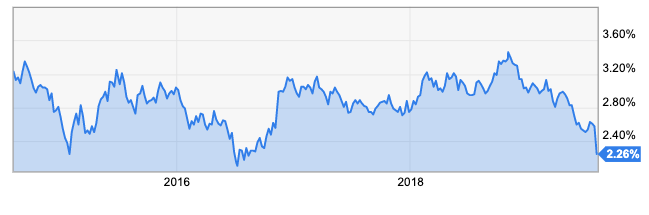
\includegraphics[width=1\textwidth]{30-year-treasury-rate-226-for-aug-09-2019.png}
    \caption{The 30 Year US Treasury Rate is 2.26\% as of Aug 09, 2019. This is well below the long term average of 5.10\% \cite{30YearTreasuryRateUS}}
\end{figure}
\FloatBarrier

According to the 2012 IRENA report, if the cost of capital (or discount rate) decreased from 10\% to 3\%, the LCOE costs are approximately cut in half. \cite{RenewableEnergyTechnologiesCostAnalysisSeries} This could reduce our estimated levelized power cost of a large hydro plant to about \$0.01/kWh down from our previous low of \$0.02/kWh.

\subsection{UPHS Estimates: Utilization of Existing Dams}
Above, we estimated the total install cost of UPHS to be about \$1,300/kW. However, it could be possible to lower this cost by adding UPHS to an existing dam. In the 2017 IRENA report, the typical install costs for hydropower projects are estimated in a large range: from a low of \$500/kW to a high of around \$4,500/kW. And the report estimates that a plant built onto an existing dam could cost as low as \$450/kW.

\begin{figure}[ht!]
    \centering
    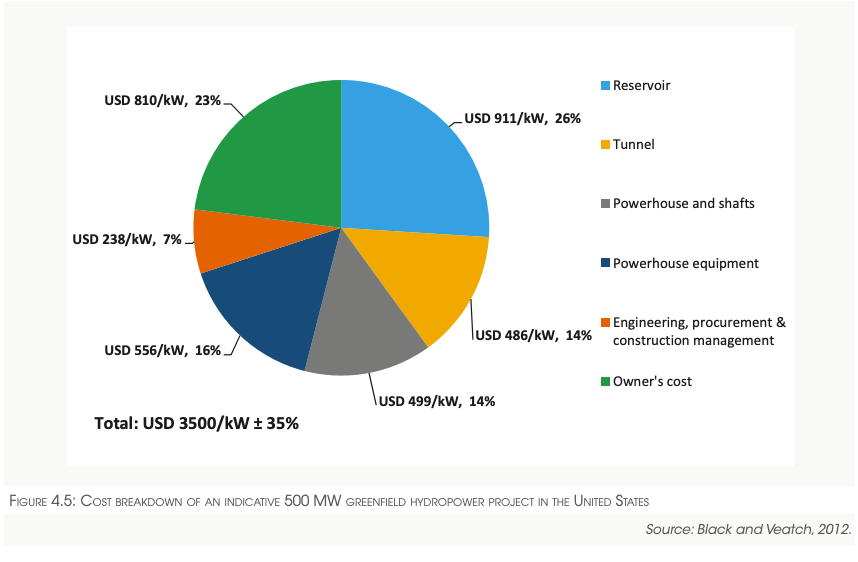
\includegraphics[width=1\textwidth]{cost-breakdown-of-typical-hydro-plant.png}
    \caption{Cost breakdown of a typical greenfield hydropower project in the US \cite{RenewableEnergyTechnologiesCostAnalysisSeries}}
\end{figure}
\FloatBarrier

As shown in the pie chart above, these savings would presumably come from reducing the 26\% reservoir costs of a greenfield development.

If we presume that a UPHS facility could benefit from similar savings, we can deduct 25\% from our previous UPHS construction estimate of \$1.3 Billion. This gives us a construction cost of \$975 Million.
\[ \$1,300,000,000 - (\$1,300,000,000 * .25) \approx \$975,000,000\]

\subsection{UPHS Estimates: Cheaper Tunnel Costs}
It's estimated that about 30\% of overall UPHS project costs are spent on digging the lower reservoir. The vertical shafts are comparably small in volume and should not add much more digging cost. \textit{See Appendix: Calculation of Vertical Shaft Volume and Cost}

As cited above, Elon Musk's Boring Company has been developing improved tunneling machines which have the potential to drastically reduce the time and cost of mining. The Boring Company claims that their technology will soon add a 10-15-fold performance gains. Although these claims certainly cannot be taken on faith without rigorous demonstration, it does make sense that performance gains should follow from the process streamlining that the company is developing. For the sake of argument, we'll choose an optimistic estimation that digging could become five times faster and cheaper than it was at the time of the 1984 PNL report when UPHS costs were calculated.

\subsection{UPHS Calculated Optimistic Estimated Cost}
With the optimistic figures above, we can re-calculate a potential lower cost of UPHS than our initial calculation. The full details of this calculation can be found in the appendix. \textit{See Appendix: Calculation of LCOE for UPHS (Optimistic)}.

\begin{displayquote}
Our calculations show that under optimistic market conditions, it's feasible that a 1,000 MW UPHS installation could have an LCOE of about \$0.015/kW, or 1.5\cent /kW.
\end{displayquote}

Again, we stress that this estimation includes some speculative assumptions. And more research is needed to attach more confidence to this number. But if any of our optimistic assumptions prove correct and UPHS could drop from a LCOE of 6.3\cent /kW to a price closer to 1.5\cent /kW, it would be extremely competitive, making it much easier for wind and solar growth to capture market share well past 50\% of the energy market.

\pagebreak[1]
\section{UPHS Versus Lithium Ion Chemical Batteries}
In the section above called \textit{Why Energy Storage?}, we discussed some of the problems with Li-ion chemical batteries and why they might not be suited for grid-scale energy storage. In this section, we'll explore this question in more detail. And we'll demonstrate why UPHS could be a far cheaper alternative.

The BloombergNEF research team recently published their Energy Outlook 2019 Report. The report's summary cites that the levelized cost of (Li-ion battery) storage will fall from today's \$187/MWh cost to around \$67/MWh by 2040. \cite{NewEnergyOutlook2019Report} They predict: “By the mid-2020s, batteries are the most cost-competitive source of peaking generation. By 2030, they challenge the duopoly of coal and gas for the provision of dispatchable generation – so producing when the sun does not shine and the wind does not blow.” \cite{NewEnergyOutlook2019Report}

But these levelized costs are much higher than those for PHS or UPHS.
Today's cost of \$187/MWh (\$0.187/kwh) is about three times more expensive than our more conservative estimate for UPHS at \$0.063/kW. And even by 2040, the cost of Li-ion batteries would still be more expensive at \$67/MWh (\$0.067/kW) than our conservative estimate for UPHS at \$0.063/kW.

But it gets worse. Li-ion battery life has a max of 7-10 years at best, and degrades steadily even in early years. \cite{LifePredictionModelForLiIonBattery}

In the article above about the Hoover dam, the New York Times quotes chemistry professor Sri Narayan who believes lifespans are likely even shorter in the real world. He said, “With lithium-ion batteries, you have durability issues...If they last five to 10 years, that would be a stretch, especially because we expect to use these facilities at full capacity.” \cite{The3BillionPlanToTurnHooverDamIntoAGiantBattery}

\begin{figure}[ht!]
    \centering
    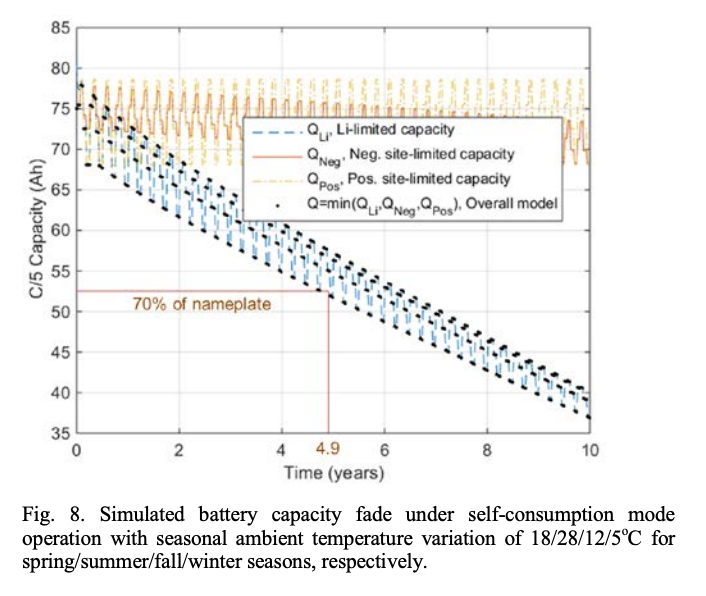
\includegraphics[width=.75\textwidth]{li-ion-battery-life.png}
    \caption{Battery Life for Grid-Scale Li-Ion Batteries \cite{LifePredictionModelForLiIonBattery}}
\end{figure}
\FloatBarrier

With a 5-10 year lifespan, a LCOE of \$67/MWh for Li-ion by 2040 looks much less enticing. Because this means that the equivalent LCOE for a 40 year operating storage plant would be at least \$268/MWh for Li-ion. Over 80 years, it could be \$536/MWh. Since the lifespan of a UPHS facility can exceed 80 years, the LCOE of UPHS does not change over that same time.

\begin{displayquote}
Even if the cost of Li-ion batteries is cut in half by 2040, we still estimate UPHS storage to be cheaper than Li-ion battery storage by an order of magnitude. Over 80 years, Li-ion is estimated to cost at least 8 times more than UPHS (\$536/MWh vs \$67/MWh). Under optimistic conditions favoring UPHS, UPHS could be 35 times cheaper than Li-ion over 80 years. (\$536/MWh vs \$15/MWh)
\end{displayquote}

And, we have further problems with Li-ion batteries. Researchers are not even sure that our planet can supply all the materials needed to produce enough batteries. According to research by the University of Technology Sydney, by 2050, “demand from renewable energy and storage technologies could exceed reserves for cobalt, lithium and nickel, and reach 50\% of reserves for indium, silver, tellurium.”

\begin{figure}[ht!]
    \centering
    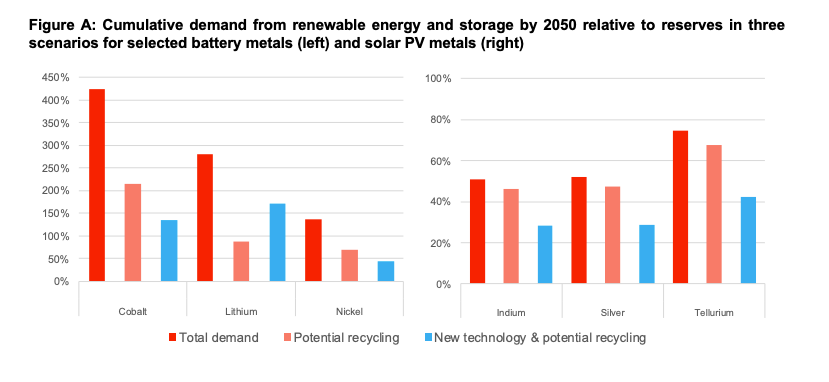
\includegraphics[width=1\textwidth]{chemical-battery-reserves-for-2050.png}
    \caption{Cumulative demand from renewable energy and storage by 2050 relative to reserves -  UTS 2019 \cite{ResponsibleMineralsSourcingForRenewableEnergy}}
\end{figure}
\FloatBarrier

According to that report (Institute for Sustainable Futures report), some materials will experience a threatened supply even sooner.

\begin{displayquote}
“The rapid increase in demand for cobalt, lithium and rare earths is of the most concern. Demand for lithium and rare earths from lithium-ion batteries for EVs and storage exceeds current production rates by 2022 (for all uses).” \cite{ResponsibleMineralsSourcingForRenewableEnergy}
\end{displayquote}

Furthermore, chemical batteries are a known source of pollution. It will be  important to monitor and better understand the repercussions of such pollution as mining increases. Here is one story highlighted by the Institute for Sustainable Futures report:

\begin{displayquote}
“Although not well documented, there have been ongoing negative social environmental impacts in China, which at one point was producing 97\% of the worlds’ supply [of rare earth ores]. The town of Baotou, in Inner Mongolia, processes rare earths from the Bayan Obo mine, a 48 square kilometre open-pit mine that is the largest source of rare earths in China, as well as producing iron ore. Here wastewater from the tailings dams has polluted groundwater, which has led to crop failures and the displacement of farming communities.” \cite{ResponsibleMineralsSourcingForRenewableEnergy}
\end{displayquote}

\subsection{UPHS Plus Lithium Ion Batteries}
Despite some downsides of Li-ion batteries, they are still a crucial technology which will help us increase global battery storage and increase renewable energy resources. As stated earlier, chemical batteries are particularly good for replacing peaker-plants on a local scale. We outline the downsides of Li-ion only to illustrate that the technology is probably not as well suited for grid-scale energy storage compared to other options.

Further, we demonstrate that underground pumped hydro energy storage could be a more effective solution than Li-ion batteries -- by an order of magnitude on long-term scales.

\pagebreak[1]
\section{Conclusion}
In this report we have explained the critical importance of building an enormous capacity of energy storage. And we have shown that underground pumped hydro storage could very well be our most affordable means of accomplishing this task. We estimate that this technology could be 8 to 35 times cheaper than Li-ion battery solutions over long time periods of 80 years.

Without overstatement, civilization is in a state of climate emergency. Our fight against climate change will demand a global, multi-faceted effort. This challenge is our generation's “moonshot mission.” But our choice is clear: If we fail to act, we doom future generations to escalating and inescapable climate damages. Or, we can invest in long-term climate solutions. If we take action and do this immediately, we have a chance to inherit a future with a healthier climate and a stronger economy.

UPHS has the potential to save billions of dollars by solving one of our most vexing climate change problems. Let's pursue further research into this technology, and let's start immediately.

\pagebreak[4]
\import{sections/}{appendix.tex}


% until today, there has simply not been enough market demand for energy storage to justify further experimentation with the idea. After all, of the 24 operational pumped storage projects in the US, most are over 30 years old.\cite{USFederalEnergyRegulatoryCommission}. Those storage plants also served a different need than we will need today. Pumped Hydro “historically has been used to balance load on a system, enabling large nuclear or thermal generating sources to operate at peak efficiencies.”\cite{ESAPumpedHydroelectricStorage}. Today, our evolving energy market looks very different. With wind and solar rapidly increasing our grid's variability, our energy storage needs are expected to soar. Energy storage will no longer be an optimizer of efficiency, it will be a dependency upon which our wind and solar markets must stake their future.

% funding ideas:
% https://www.energy.gov/eere/water/pumped-storage-hydropower
% http://energywatchgroup.org/about-us

{\footnotesize
\bibliographystyle{unsrt}
\bibliography{bibliography}
}

% \cite{ObamaIssuesChallengeOnClimateChangeWithPowerPlantRule}

% “We’re the first generation to feel the impact of climate change. We’re the last generation that can do something about it,” Obama told a sympathetic audience at the White House.

% “We only get one home. We only get one planet. There’s no plan B.”


% \begin{displayquote}
% Long quote
% \end{displayquote}

\end{document}
% “”